\documentclass[12pt,prb,aps]{revtex4-1}
\usepackage {amsmath}
\pdfoutput = 1 
\usepackage {graphicx}

\begin{document}

\title{Influence of anomalous perpendicular transport on linear tearing mode dynamics in tokamak plasmas}

\author{R.~Fitzpatrick\,\footnote{rfitzp@utexas.edu}}
\affiliation{Institute for Fusion Studies,  Department of Physics,  University of Texas at Austin,  Austin TX, 78712, USA}

\begin{abstract}
The analysis of a previous paper [A.~Cole, and R.~Fitzpatrick, Phys.\ Plasmas {\bf 13}, 032503 (2006)] that maps out all of the
two-fluid response regimes of a  linear tearing layer interacting with an externally generated resonant magnetic perturbation, in a large aspect-ratio tokamak plasma,  is generalized to
take into account realistic levels of perpendicular particle transport. A new response-regime map is obtained that differs substantially, in many
respects, from the old one. The improved analysis is first employed to find all of the two-fluid growth-rate regimes of a non-interacting low-mode-number tearing mode in a large aspect-ratio tokamak plasma. 
The analysis is then used to determine the scaling of the error-field penetration threshold with machine
parameters in large aspect-ratio tokamak plasmas. 
\end{abstract}

\maketitle

\section{Introduction}
Tearing modes are slowly growing instabilities of ideally-stable tokamak plasmas that reconnect magnetic field-lines
at various resonant surfaces within the plasma, in the process forming magnetic island chains that degrade the plasma confinement.\cite{wes}
If tearing modes grow to sufficiently large amplitude then they can trigger major disruptions.\cite{wes1}  Tokamak
plasmas are observed to be particularly disruption-prone when tearing modes {\em lock}\/ (i.e., become stationary in the
laboratory frame) to externally generated, resonant magnetic perturbations.\cite{vries}  

It is well known that single-fluid, resistive magnetohydrodynamics (MHD) offers a very poor description of
tearing mode dynamics in tokamak plasmas. 
For instance, the strong {\em diamagnetic}\/ flows present in such plasmas decouple the electron and ion flows to some extent,
necessitating a two-fluid treatment.\cite{ara} Moreover, resistive-MHD does not take  the important {\em ion sound radius} lengthscale, below which electron and ion dynamics are further decoupled, 
into account.\cite{drake,wal} Previously, Cole \& Fitzpatrick\,\cite{cole} used the four-field model
of Fitzpatrick \& Waelbroeck\,\cite{fw} (which is based on the original four-field model of Hazeltine, et al.\cite{haz}) 
to determine the two-fluid response of a linear tearing layer to an externally generated, 
resonant magnetic perturbation  in a large aspect-ratio tokamak plasma. However, the treatment of Cole \& Fitzpatrick fails to take into account the
 anomalously large perpendicular  particle diffusivity  present in tokamak plasmas. The
aim of this paper is to correct this deficiency. 

This paper is organized as follows. After some preliminary analysis in Sect.~\ref{sect1}, our fundamental four-field resonant
plasma response model is introduced in Sect.~\ref{sfour}. This model is a slightly improved version of the model derived in Ref.~\onlinecite{fw} that takes the thermal force into account. (The thermal force merely gives rise to an additional term  in the perpendicular electron fluid velocity that scales as the electron temperature gradient.) The model is converted into a set of linear layer equations in
Sect.~\ref{layer}. These layer equations are then solved in Sect.~\ref{linear} in order to map out all of the linear response regimes
of a resonant layer to an externally generated, resonant magnetic perturbation in a large aspect-ratio tokamak plasma. In Sect.~\ref{stab}, we reuse the analysis of Sect.~\ref{linear} to map out all
of the growth-rate regimes for a low-mode-number (but not $m=1$) tearing mode in a large aspect-ratio tokamak plasma. Finally,
in Sect.~\ref{error}, we employ the results of Sect.~\ref{linear} to determine the scaling of the error-field penetration threshold with machine parameters
 in large aspect-ratio tokamak plasmas. 

\section{Preliminary Analysis}\label{sect1}
\subsection{Plasma Equilibrium}
Consider a large aspect-ratio tokamak plasma equilibrium whose magnetic flux-surfaces map out
(almost) concentric circles in the poloidal plane. Such an equilibrium can be approximated as a
periodic cylinder.\cite{rf1993} Let $r$, $\theta$, $z$ be right-handed cylindrical coordinates. 
The magnetic axis corresponds to $r=0$, and the plasma boundary to $r=a$. The system is assumed to be periodic in the $z$
direction with periodicity length $2\pi\,R_0$, where $R_0$ is the simulated major radius of the plasma. The
safety-factor profile takes the form $q(r)=r\,B_z/[R_0\,B_\theta(r)]$, where $B_z$ is the constant
`toroidal' magnetic field-strength, and $B_\theta(r)$ is the poloidal magnetic field-strength. The standard
large aspect-ratio orderings, $r/R_0\ll 1$ and $B_\theta/B_z\ll 1$, are adopted. 

\subsection{Asymptotic Matching}\label{cyl}
Consider a tearing mode perturbation that has $m$ periods in the poloidal direction, and
$n$ periods in the toroidal direction. 
As is well known, the response of the plasma to the tearing mode is
governed by marginally stable, ideal-MHD everywhere in the plasma, apart from a (radially) narrow
layer centered on the so-called {\em resonant surface}, minor radius $r_s$, at which $q(r_s)=m/n$.\cite{fkr}

The perturbed magnetic field associated with the tearing mode is written $\delta{\bf B} \simeq \nabla\delta\psi\times{\bf e}_z$,  
where
$\delta\psi(r,\theta,\varphi,t)= \delta\psi(r,t)\,\exp[\,{\rm i}\,(m\,\theta-n\,\varphi)]$, 
and $\varphi=z/R_0$ is a simulated toroidal angle. 

In the so-called {\em outer region}\/ (i.e., everywhere in the plasma
apart from the resonant layer), the perturbed helical magnetic flux, $\delta\psi(r,t)$, satisfies the
{\em cylindrical tearing mode equation}:\cite{wes}
\begin{equation}\label{e3}
\frac{\partial^2\delta\psi}{\partial r^2} + \frac{1}{r}\,\frac{\partial\delta\psi}{\partial r}-\frac{m^2}{r^2}\,\delta\psi - \frac{J_z'\,\delta\psi}{r\,(1/q-n/m)}=  0,
\end{equation}
where 
$J_z(r)= R_0\,\mu_0\,j_z(r)/B_z$,
and $j_z(r)$ is the equilibrium `toroidal' current density. Here, $'\equiv d/dr$. In general, the solution of Eq.~(\ref{e3}) that satisfies physical
boundary conditions at the magnetic axis and the plasma boundary is such that $\delta\psi$ is continuous
across the resonant surface, whereas $\partial\delta\psi/\partial r$ is discontinuous. The discontinuity of
 $\partial\delta\psi/\partial r$ across the resonant surface is indicative of the presence of a helical current
 sheet at the surface.  The complex quantity ${\mit\Psi}_s(t)= \delta\psi(r_s,t)$ determines the amplitude
 and phase of the reconnected helical magnetic flux at the resonant surface, whereas the complex quantity\,\cite{rf1993}
 \begin{equation}
{\mit\Delta\Psi}_s = \left[r\,\frac{\partial \delta\psi}{\partial r}\right]_{r_{s-}}^{r_{s+}}
\end{equation}
parameterizes the amplitude and phase of the helical current sheet flowing at the surface. The solution of
the cylindrical tearing mode equation in the outer region, in the presence of an externally generated, resonant magnetic perturbation 
of the same helicity as the tearing mode, leads to the relation\,\cite{rf1993,fkr}
\begin{equation}\label{e110}
{\mit\Delta\Psi}_s= ({\mit\Delta}_s')\,{\mit\Psi}_s + (-{\mit\Delta}_s')\,{\mit\Psi}_v,
\end{equation}
where ${\mit\Delta}_s'$ is a real dimensionless quantity known as the {\em tearing stability index}. Moreover,
${\mit\Psi}_v$ is the so-called {\em vacuum flux}, and is defined as the reconnected magnetic flux
that would be driven at the resonant surface by the resonant magnetic perturbation were the
plasma intrinsically tearing stable (i.e., ${\mit\Delta}_s' <0$), and were there no current sheet at the resonant surface
(i.e., ${\mit\Delta\Psi}_s=0$).

The current sheet at the resonant surface can only be resolved by solving  a two-fluid, resistive-MHD, plasma response model
in the so-called {\em inner region}\/ (i.e., the region of the plasma in the immediate vicinity of the resonant surface), 
and asymptotically matching the solution so obtained to the ideal-MHD solution in the outer region. The particular 
plasma response model used in this paper is
described in the following section. 

\section{Four-Field Resonant Plasma Response Model}\label{sfour}
\subsection{Useful Definitions}
The plasma is assumed to consist of two species. First, electrons of mass $m_e$, electrical charge $-e$, 
number density $n$, and temperature $T_e$.  Second, ions of mass $m_i$, electrical charge $+e$,  
number density $n$, and temperature $T_i$. Let $p=n\,(T_e+T_i)$ be the total plasma pressure. 

It is helpful to define $n_0 = n(r_s)$, $p_0= p(r_s)$,
\begin{align}
\eta_e &=\left.\frac{d\ln T_e}{d\ln n}\right|_{r=r_s},\label{e211}\\[0.5ex]
\eta_i &= \left.\frac{d\ln T_i}{d\ln n}\right|_{r=r_s},\\[0.5ex]
\tau &= \left(\frac{T_e}{T_i}\right)_{r=r_s}\left(\frac{1+\eta_e}{1+\eta_i}\right),\label{e213}
\end{align}
where $n(r)$, $p(r)$, $T_e(r)$, and $T_i(r)$ refer to
density, pressure, and temperature profiles that are unperturbed by the tearing mode. 

For the sake of simplicity, the perturbed electron and ion temperature profiles are assumed to be functions of
the perturbed electron number density profile in the immediate vicinity of the resonant surface. In other words, $T_e=T_e(n)$ and $T_i=T_i(n)$. This
implies that $p=p(n)$. 
The {\em MHD velocity}, which is the velocity of a
fictional MHD fluid, is defined ${\bf V}={\bf V}_E + V_{\parallel\,i}\,{\bf b}$, where ${\bf V}_E$ is the
${\bf E}\times{\bf B}$ drift velocity, $V_{\parallel\,i}$ is the parallel component of the ion fluid
velocity, ${\bf b}= {\bf B}/|{\bf B}|$, and ${\bf B}$ is the magnetic field-strength.

\subsection{Fundamental Fields}
The four fundamental fields in our four-field model---namely, $\psi$, $\phi$, $N$, and $V$---have the following
definitions:
\begin{align}\label{e10}
\nabla\psi &= \frac{{\bf n}\times{\bf B}} {r_s\,B_z},\\[0.5ex]
\nabla\phi &= \frac{{\bf n}\times {\bf V}}{r_s\,V_A},\\[0.5ex]
N &=-\hat{d}_i\left(\frac{p-p_0}{B_z^{\,2}/\mu_0}\right),\\[0.5ex]
V &= \hat{d}_i\left(\frac{{\bf n}\cdot {\bf V}}{V_A}\right).\label{e13}
\end{align}
Here,   ${\bf n} = (0,\,\epsilon/q_s,\,1)$, $\epsilon = r/R_0$, $q_s=m/n$, 
$V_A =B_z/\sqrt{\mu_0\,n_0\,m_i}$, 
$d_i = \sqrt{m_i/(n_0\,e^{\,2}\,\mu_0)}$,
and $\hat{d}_i=d_i/r_s$. 
 Our
model also employs the auxiliary field
\begin{align}\label{e16}
J=-\frac{2\,\epsilon_s}{q_s}+\hat{\nabla}^2\psi,
\end{align}
where 
$\epsilon_s=r_s/R_0$, and $\hat{\nabla} = r_s\,\nabla$. 

\subsection{Fundamental Equations}
The four-field model takes the form:\cite{fw}
\begin{align}
\frac{\partial\psi}{\partial\hat{t}}&= [\phi,\psi] -\tau_e\,(1+\lambda_e)\,[N,\psi]
+\hat{\eta}_\parallel\,J + \hat{E}_\parallel,\\[0.5ex]
\frac{\partial \hat{\nabla}^2\phi}{\partial \hat{t}}&= [\phi,\hat{\nabla}^2\phi] - \frac{\tau_i}{2}\left(\hat{\nabla}^2[\phi,N] + [\hat{\nabla}^2\phi,N] + [\hat{\nabla}^2 N,\phi]\right) + [J,\psi] \nonumber\\[0.5ex]&\phantom{=}+\hat{\chi}_\varphi  \,\hat{\nabla}^4\!\left(\phi + \tau_i\,N\right), \\[0.5ex]
\frac{\partial N}{\partial \hat{t}}&= [\phi,N] +c_\beta^{\,2}\,[V,\psi] +\hat{d}_\beta^{\,2}\,[J,\psi]
+ \hat{D}_\perp\,\hat{\nabla}_\perp^{\,2}N,\\[0.5ex]
\frac{\partial V}{\partial\hat{t}}&= [\phi,V] +[N,\psi] + \hat{\chi}_\varphi\,\hat{\nabla}^2 V.\label{e21}
\end{align}
Here, $[A,B]\equiv \hat{\nabla} A\times \hat{\nabla} B\cdot {\bf n}$, $\tau_e=[\tau/(1+\tau)]$, $\tau_i=1/(1+\tau)$, $\hat{t} = t/(r_s/V_A)$, $\hat{\eta}_{\parallel,\perp} = \eta_{\parallel,\perp}/(\mu_0\,r_s\,V_A)$, $\hat{E}_\parallel = E_\parallel/(B_z\,V_A)$, 
$\hat{\chi}_\varphi= \chi_\varphi/(r_s\,V_A)$, where $\eta_{\parallel,\perp}$ is the parallel/perpendicular plasma electrical
resistivity at the resonant surface, $E_\parallel$ the parallel inductive electric field that maintains the equilibrium toroidal
plasma current in the vicinity of the resonant surface, and $\chi_\varphi$  the anomalous perpendicular ion momentum
diffusivity at the resonant surface. 
Moreover, $d_\beta=c_\beta\,d_i$, and $\hat{d}_\beta=d_\beta/r_s$, where $c_\beta = \sqrt{\beta/(1+\beta)}$, and
$\beta=(5/3)\,\mu_0\,p_0/B_z^{\,2}$. Here, $d_\beta$ is usually referred to as the {\em ion sound radius}. Furthermore,
$\lambda_e=0.71\,\eta_e/(1+\eta_e)$ originates from the thermal force. Finally,\cite{fw}
\begin{equation}
\hat{D}_\perp \equiv \frac{D_{\perp}}{r_s\,V_A}= c_\beta^{\,2}\,\hat{\eta}_\perp +  \frac{2}{3}\left(1-c_\beta^{\,2}\right)\!\left(\frac{\eta_e\,\tau_e}{1+\eta_e}\,\hat{\chi}_{\perp\,e} + \frac{\eta_i\,\tau_i}{1+\eta_i}\,\hat{\chi}_{\perp\,i}\right),
\end{equation}
where $\hat{\chi}_{\perp\,e,i}=\chi_{\perp\,e,i}/(r_s\,V_A)$, and $\chi_{\perp\,e,i}$ is the (anomalous)
perpendicular electron/ion  energy diffusivity in the vicinity of the resonant surface. 
Note that Cole \& Fitzpatrick (2006) neglects the contribution of $\chi_{\perp\,e,i}$ to the perpendicular particle
diffusivity, $D_\perp$, leading to an anomalously small estimate for $D_\perp$. It is this deficiency that we aim to
correct in the present paper. To be more exact, given that $c_\beta\ll 1$ in conventional tokamak plasmas, and
that $\hat{\eta}_\perp\ll \hat{\chi}_{\perp\,e,i}$ (i.e., magnetic flux typically diffuses  across magnetic flux surfaces in tokamak plasmas much more
slowly than energy), the neglect of the terms involving $\hat{\chi}_{\perp\,e,i}$ in the previous equation leads to the
erroneous conclusion that $\hat{D}_\perp\ll \hat{\chi}_{\perp\,e,i}$ (i.e., particles diffuse across magnetic flux-surfaces in tokamak plasmas 
much more slowly than energy). The inclusion of the terms leads to the correct conclusion that  $\hat{D}_\perp\sim \hat{\chi}_{\perp\,e,i}$ (i.e., particles diffuse across magnetic flux-surfaces 
at a similar rate to energy). 

\subsection{Matching to Plasma Equilibrium}
The unperturbed plasma equilibrium is such that
${\bf B} = (0,\,B_\theta(r),\,B_z)$,  $p = p(r)$,
${\bf V} = (0,\,V_E(r),\,V_z(r))$,
where 
$V_E(r)\simeq E_r/B_z$
 is the (dominant $\theta$-component of the) ${\bf E}\times {\bf B}$ velocity. Now, the resonant layer is assumed to have a radial thickness that is
much smaller than $r_s$.   Hence, we only need to evaluate plasma equilibrium quantities in the immediate vicinity of the resonant
surface. Equations~(\ref{e10})--(\ref{e13}) suggest that 
\begin{align}
\psi&= \frac{\hat{x}^{\,2}}{2\,\hat{L}_s},\label{e23}\\[0.5ex]
\phi &= - \hat{V}_E\,\hat{x},\\[0.5ex]
N &= -\hat{V}_\ast\,\hat{x},\\[0.5ex]
V &= \hat{V}_\parallel,\label{e26}
\end{align}
where 
$\hat{x}=(r-r_s)/r_s$,
 $\hat{L}_s=L_s/r_s$,  $L_s=R_0\,q_s/s_s$, 
  $\hat{V}_E= V_E(r_s)/V_A$,
$\hat{V}_\ast= V_\ast(r_s)/V_A$,
$V_\ast(r) = (dp/dr)/(e\,n_0\,B_z)$ 
is the (dominant $\theta$-component of the) diamagnetic velocity,
  and 
 $\hat{V}_\parallel=\hat{d}_i\, V_z(r_s)/V_A$. Here, $s_s=s(r_s)$ and $s(r)=d\ln q/d\ln r$. We also have
 \begin{align}\label{e28}
 J &= -\left(\frac{2}{s_s}-1\right)\frac{1}{\hat{L}_s},
\end{align} 
and $ \hat{E}_\parallel =(2/s_s-1) (\hat{\eta}_\parallel/\hat{L}_s)$.

\section{Linear Resonant Plasma Response Model}\label{layer}
\subsection{Introduction}
The aim of this section is to obtain a set of linear layer equations from the four-field model
introduced in Sect.~\ref{sfour}.

\subsection{Derivation of Linear Layer Equations}
In accordance with Eqs.~(\ref{e23})--(\ref{e28}), let us write
\begin{align}\label{e31}
\psi(\hat{x},\zeta,\hat{t}) &= \frac{\hat{x}^{\,2} }{2\,\hat{L}_s}+ \tilde{\psi}(\hat{x})\,{\rm e}^{\,{\rm i}\,(\zeta-\hat{\omega}\,\hat{t})},\\[0.5ex]
\phi(\hat{x},\zeta,\hat{t}) &=-\hat{V}_E\,\hat{x}+ \tilde{\phi}(\hat{x})\,{\rm e}^{\,{\rm i}\,(\zeta-\hat{\omega}\,\hat{t})},\\[0.5ex]
N(\hat{x},\zeta,\hat{t}) &= -\hat{V}_\ast\,\hat{x}+\tau_e\,\tilde{N}(\hat{x})\,{\rm e}^{\,{\rm i}\,(\zeta-\hat{\omega}\,\hat{t})},\\[0.5ex]
V(\hat{x},\zeta,\hat{t}) &= \hat{V}_\parallel +\tau_e\,\tilde{V}(\hat{x})\,{\rm e}^{\,{\rm i}\,(\zeta-\hat{\omega}\,\hat{t})},\\[0.5ex]
J(\hat{x},\zeta,\hat{t}) &=-\left(\frac{2}{s_s}-1\right)\!\frac{1}{\hat{L}_s}+ \hat{\nabla}^2\tilde{\psi}(\hat{x})\,{\rm e}^{\,{\rm i}\,(\zeta-\hat{\omega}\,\hat{t})},\label{e36}
\end{align}
where $\zeta=m\,\theta-n\,\varphi$, $\hat{\omega}=r_s\,\omega/V_A$, and $\omega$ is the frequency of the tearing mode in the laboratory frame. 
Substituting Eqs.~(\ref{e31})--(\ref{e36}) into Eqs.~(\ref{e16})--(\ref{e21}), 
 and only retaining terms that
are first order in perturbed quantities, we obtain the following set of linear equations:
\begin{align}\label{e37}
-{\rm i}\,[\omega-\omega_E -(1+\lambda_e)\,\omega_{\ast\,e}]\,\tau_H\,\tilde{\psi} &= -{\rm i} \,\hat{x}\,[\tilde{\phi}-(1+\lambda_e)\,\tilde{N}] + S^{-1}\,\hat{\nabla}^2\tilde{\psi},\\[0.5ex]
-{\rm i}\,(\omega-\omega_E-\omega_{\ast\,i})\,\tau_H\,\hat{\nabla}^2\tilde{\phi} &= -{\rm i}\,\hat{x}\,\hat{\nabla}^2\tilde{\psi}+S^{-1}\,P_\varphi\,\hat{\nabla}^4\!\left(\tilde{\phi} + \frac{\tilde{N}}{\tau}\right),\\[0.5ex]
-{\rm i}\,(\omega-\omega_E)\,\tau_H\,\tilde{N} &= -{\rm i}\,\omega_{\ast\,e}\,\tau_H\,\tilde{\phi}-{\rm i}\,c_\beta^{\,2}\,\hat{x}\,\tilde{V} - {\rm i}\,\tau_e\,\hat{d}_\beta^{\,2}\,\hat{x}\,\hat{\nabla}^2\tilde{\psi}\nonumber\\[0.5ex]
&\phantom{=} + S^{-1}\,P_\perp\,\hat{\nabla}_\perp^2 \tilde{N},\\[0.5ex]
-{\rm i}\,(\omega-\omega_E)\,\tau_H\,\tilde{V} &= {\rm i}\,\omega_{\ast\,e}\,\tau_H\,\tilde{\psi} - {\rm i}\,\hat{x}\,\tilde{N}
+ S^{-1}\,P_\varphi\,\hat{\nabla}^2\tilde{V}.\label{e40}
\end{align}
Here, 
$\tau_H = L_s/(m\,V_A)$ 
is the  hydromagnetic time, 
$\omega_E =(m/r_s)\,V_E(r_s)$
  the 
 ${\bf E}\times {\bf B}$ frequency, 
$\omega_{\ast\,e} = -\tau_e\,(m/r_s)V_\ast(r_s)$
the 
   electron diamagnetic
frequency,
$\omega_{\ast\,i} =\tau_i\,(m/r_s)V_\ast(r_s)$
 the  ion diamagnetic
frequency, 
$S=\tau_R/\tau_H$
 the  Lundquist number, 
$\tau_R = \mu_0\,r_s^{\,2}/\eta_\parallel$
 the
 resistive diffusion time, 
$\tau_\varphi
= r_s^{\,2}/\chi_\varphi$
the  toroidal momentum confinement time, and 
$\tau_\perp = r_s^{\,2}/D_\perp$.
  Furthermore, $P_\varphi = \tau_R/\tau_\varphi$ and $P_\perp = \tau_R/\tau_\perp$ are magnetic Prandtl numbers.

 Let us define the stretched radial variable $X = S^{1/3}\,\hat{x}$.
Assuming that $X\sim{\cal O}(1)$ in the layer (i.e., assuming that the layer thickness is roughly of order $S^{-1/3}\,r_s$),
and making use of the fact that $S\gg 1$ in conventional tokamak plasmas,  Eqs.~(\ref{e37})--(\ref{e40}) reduce to the following
set of linear layer equations:\,\cite{cole}
\begin{align}\label{e43}
-{\rm i}\,[Q-Q_E-(1+\lambda_e)\,Q_{e}]\,\tilde{\psi}&= - {\rm i}\,X\left[\tilde{\phi}-(1+\lambda_e)\,\tilde{N}\right] + \frac{d^{\,2}\tilde{\psi}}{d X^2},\\[0.5ex]
-{\rm i}\,(Q-Q_E -Q_{i})\,\frac{d^{\,2}\tilde{\phi}}{dX^2}&= - {\rm i}\,X\,\frac{d^{\,2}\tilde{\psi}}{dX^2}+ P_\varphi\,\frac{d^{\,4}}{dX^4}\!\left(\tilde{\phi} + \frac{\tilde{N}}{\tau}\right),\\[0.5ex]
-{\rm i}\,(Q-Q_E)\tilde{N} &= - {\rm i}\,Q_{e}\,\tilde{\phi} - {\rm i}\,c_\beta^{\,2}\,X\,\tilde{V}  - {\rm i} \,D^{2}\,X\,\frac{d^{\,2}\tilde{\psi}}{dX^{2}}
+ P_\perp\,\frac{d^{\,2} \tilde{N}}{dX^{2}},\\[0.5ex]
 -{\rm i}\,(Q-Q_E)\,\tilde{V} &= {\rm i}\,Q_{e}\,\tilde{\psi} - {\rm i}\,X\,\tilde{N} + P_\varphi\,\frac{d^{\,2}\tilde{V}}{dX^{2}}.\label{e46}
\end{align}
Here, $Q=S^{\,1/3}\,\omega\,\tau_H$, $Q_E = S^{\,1/3}\,\omega_E\,\tau_H$, $Q_{e,i} = S^{\,1/3}\,\omega_{\ast\,e,i}\,\tau_H$,
and $D = S^{\,1/3}\,\tau_e^{1/2}\,\hat{d}_\beta$. 

\subsection{Asymptotic Matching}
The  linear layer equations, (\ref{e43})--(\ref{e46}), possess tearing parity solutions
characterized by the symmetry $\tilde{\psi}(-X)=\tilde\psi(X)$, $\tilde{\phi}(-X)=-\tilde{\phi}(X)$, 
$\tilde{N}(-X)= - \tilde{N}(X)$, $\tilde{V}(-X)=\tilde{V}(X)$. If we assume that
the asymptotic behavior of the tearing parity layer solutions is such that 
\begin{equation}\label{e47}
\tilde{\psi}\rightarrow  \psi_0\!\left[1+ \frac{\hat{\mit\Delta}}{2}\,|X| + {\cal O}(X^2)\right]
\end{equation}
as $|X|\rightarrow\infty$, where $\psi_0$ is an arbitrary constant, then asymptotic matching to the outer solution yields
\begin{equation}\label{e48}
{\mit\Delta\Psi}_s= (S^{1/3}\,\hat{\mit\Delta})\,\,{\mit\Psi}_s.
\end{equation}

\section{Linear Resonant Plasma Response Regimes}\label{linear}
\subsection{Introduction}
The aim of this section is to solve the linear layer equations derived in Sect.~\ref{layer} to determine the
response of a resonant layer to an external perturbation. 

\subsection{Fourier Transformation}
Equations~(\ref{e43})--(\ref{e46}) are most conveniently solved in Fourier transform space.\cite{cole} 
Let
\begin{equation}
\bar{\phi}(p) = \int_{-\infty}^\infty \tilde{\phi}(X)\,{\rm e}^{-{\rm i}\,p\,X}\,dX,
\end{equation}
et cetera. The Fourier transformed linear layer equations become
\begin{align}\label{e314}
-{\rm i}\,[Q-Q_E-(1+\lambda_e)\,Q_{e}]\,\bar{\psi}&=\frac{d}{dp}\!\left[\bar{\phi}-(1+\lambda_e)\,\bar{N}\right] -p^2\,\bar{\psi},\\[0.5ex]
-{\rm i}\,(Q-Q_E -Q_{i})\,p^2\,\bar{\phi}&=  \frac{d(p^2\,\bar{\psi})}{dp}- P_\varphi\,p^4\!\left(\bar{\phi} + \frac{\bar{N}}{\tau}\right),\\[0.5ex]
-{\rm i}\,(Q-Q_E)\bar{N} &= - {\rm i}\,Q_{e}\,\bar{\phi} + c_\beta^{\,2}\,\frac{d\bar{V}}{dp}-D^{2}\,\frac{d(p^2\,\bar{\psi})}{dp}
  - P_\perp\,p^2\bar{N},\label{e316}\\[0.5ex]
 -{\rm i}\,(Q-Q_E)\,\bar{V} &= {\rm i}\,Q_{e}\,\bar{\psi} +\frac{d\bar{N}}{dp}- P_\varphi\,p^2\,\bar{V},\label{e317}
\end{align}
where, for a tearing parity solution, 
\begin{equation}
\bar{\phi}(p)\rightarrow \bar{\phi}_0\!\left[\frac{\hat{\mit\Delta}}{\pi\,p} + 1+ {\cal O}(p)\right]
\end{equation}
as $p\rightarrow 0$. 

Let us ignore the term $c_\beta^{\,2}\,d\bar{V}/dp$ in Eq.~(\ref{e316}). This approximation can
be justified {\em a posteriori}. It is equivalent to the neglect of the contribution of ion parallel dynamics to the linear  plasma
response in the resonant layer, and effectively decouples Eq.~(\ref{e317}) from Eqs.~(\ref{e314})--(\ref{e316}).\cite{cole,ber} Equations~(\ref{e314})--(\ref{e316}) reduce to\,\cite{cole}
\begin{equation}\label{e320}
\frac{d}{dp}\!\left[G(p)\,\frac{dY_e}{dp}\right] - \frac{A(p)}{B(p)}\,p^{2}\,Y_e = 0,
\end{equation}
where
\begin{align}
G(p)&= \frac{p^2}{-{\rm i}\,[Q-Q_E-(1+\lambda_e)\,Q_e] + p^2},\\[0.5ex]
 A(p) &= -(Q-Q_E)\,(Q-Q_E-Q_i)-{\rm i}\,(Q-Q_E-Q_i)\,(P_\varphi+P_\perp)\,p^2 + P_\varphi\,P_\perp\,p^4,\label{e45}\\[0.5ex]
 B(p) &= 
-{\rm i}\,[Q-Q_E-(1+\lambda_e)\,Q_e] +\{P_\perp - {\rm i}\,(1+\lambda_e)\,(Q-Q_E-Q_i)\,D^2\}p^2\nonumber\\[0.5ex]
&\phantom{=}+[(1+\lambda_e)+1/\tau]\,P_\varphi\,D^2\,p^4,
\end{align}
and $Y_e=\bar{\phi} - (1+\lambda_e)\,\bar{N}$. The boundary conditions are that $Y_e(p)$ is bounded as $p\rightarrow\infty$, and
\begin{equation}\label{e325}
Y_e(p)\rightarrow Y_0\!\left[\frac{\hat{\mit\Delta}}{\pi\,p} + 1+ {\cal O}(p)\right]
\end{equation}
as $p\rightarrow 0$. In the following, we shall assume that $|Q|\sim |Q_E|\sim |Q_e|\sim |Q_i|$, $P_\varphi\sim P_\perp \sim P$, $\tau\sim {\cal O}(1)$, and $\lambda_e\sim{\cal O}(1)$,  for the
sake of simplicity. 

\subsection{Constant-$\psi$ Approximation}\label{s5.6}
Let us suppose that there are two layers in $p$ space. In the small-$p$ layer, suppose that Eq.~(\ref{e320}) reduces to
\begin{equation}
\frac{d}{dp}\!\left[\frac{p^2}{-{\rm i}\,[Q-Q_E-(1+\lambda_e)\,Q_e] + p^2}\,\frac{dY_e}{dp}\right]\simeq 0
\end{equation}
when $p\sim Q^{1/2}$. Integrating directly, we find that
\begin{equation}
Y_e(p) \simeq Y_0 \left[\frac{\hat{\mit\Delta}}{\pi}\left(\frac{1}{p} + \frac{p}{{\rm i}\,[Q-Q_E-(1+\lambda_e)\,Q_e]}\right) + 1 + {\cal O}(p^2)\right]
\end{equation}
for $p\lesssim {\cal O}(Q^{1/2})$, where use has been made of Eq.~(\ref{e325}). The two-layer  approximation is
equivalent to the well-known {\em constant-$\psi$ approximation}.\cite{fkr}

In the large-$p$ layer, for  $p\gg {\cal O}(Q^{1/2})$, we obtain 
\begin{equation}\label{e329}
\frac{d^{\,2} Y_e}{dp^2} - \frac{A(p)}{B(p)}\,p^2\,Y_e\simeq 0,
\end{equation}
with $Y_e$ bounded as $p\rightarrow \infty$. Asymptotic matching to the small-$p$ layer yields the boundary
condition 
\begin{equation}\label{e330}
Y_e(p)\simeq Y_0\left\{1+ \frac{\hat{\mit\Delta}}{\pi}\,\frac{p}{{\rm i}\,[Q-Q_E-(1+\lambda_e)\,Q_e]}+ {\cal O}(p^2)\right\}
\end{equation}
as $p\rightarrow 0$. 

In the various constant-$\psi$ linear response regimes considered in Sect.~\ref{scp}, Eq.~(\ref{e329}) reduces to an
equation of the form
\begin{equation}\label{e330a}
\frac{d^{\,2}Y_e}{dp^2}- C\,p^m\,Y_e\simeq 0,
\end{equation}
where $m$ is real and non-negative, and $C$ is a complex constant. Let $Y_e=\sqrt{p}\,Z$ and $q=\sqrt{C}\,p^n/n$, where
$n=(m+2)/2$. The previous equation transforms into a modified Bessel equation of general order, 
\begin{equation}
q^2\,\frac{d^{\,2}Z}{dq^2} + q\,\frac{dZ}{dq} - (q^2+\nu^2)\,Z =0,
\end{equation}
where $\nu=1/(m+2)$. The solution that is bounded as $q\rightarrow \infty$ has the small-$q$
expansion
\begin{equation}\label{e332}
K_\nu(q)= \frac{1}{{\mit\Gamma}(1-\nu)}\left(\frac{2}{q}\right)^\nu - \frac{1}{{\mit\Gamma}(1+\nu)}\left(\frac{q}{2}\right)^\nu + {\cal O}(q^{2-\nu}),
\end{equation}
where ${\mit\Gamma}(z)$ is a gamma function. 
A comparison of this expression with Eq.~(\ref{e330}) reveals that
\begin{equation}
\hat{\mit\Delta} = \pi\,(-{\rm i}\,\left[Q-Q_E-(1+\lambda_e)\,Q_e\right])\, \frac{{\mit\Gamma}(1-\nu)}{{\mit\Gamma}(\nu)}\,\nu^{2\nu-1}\,C^{\,\nu}.
\end{equation}
Note, finally, that $p_\ast\sim |C|^{-\nu}$, where $p_\ast$ denotes the width of the large-$p$ layer in $p$ space. This width must be larger than $Q^{1/2}$ (i.e., the width of the small-$p$ layer) in order for the constant-$\psi$ approximation to hold. 

\subsection{Constant-$\psi$ Linear Response Regimes}\label{scp}
Suppose that $Q\gg P\,p^2$ and $D^2\,p^2 \ll 1$. It follows that $\nu=1/4$ and
\begin{equation}
C = \frac{[-{\rm i}\,(Q-Q_E)]\,[-{\rm i}\,(Q-Q_E-Q_i)]}{-{\rm i}\,[Q-Q_E-(1+\lambda_e)\,Q_e]}.
\end{equation}
Hence, we deduce that
\begin{equation}\label{ri}
\hat{\mit\Delta} = \frac{2\pi\,{\mit\Gamma}(3/4)}{{\mit\Gamma}(1/4)}\,(-{\rm i}\,[Q-Q_E-(1+\lambda_e)\,Q_e])^{3/4}\,[-{\rm i}\,(Q-Q_E)]^{1/4}\,[-{\rm i}\,(Q-Q_E-Q_i)]^{1/4}.
\end{equation}
This response regime is known as the {\em resistive-inertial regime}, because the layer response is dominated by
plasma resistivity and ion inertia.\cite{fkr,ara,rf1998}. The characteristic layer width is $p_\ast \sim Q^{-1/4}$,
which implies that the regime is valid when $P\ll Q^{3/2}$, $Q\gg D^4$, and $Q\ll 1$. 

Suppose that $Q\ll P\,p^2$ and $D^2\,p^2\ll 1$. It follows that $\nu=1/6$ and $C=P_\varphi$. 
Hence, we deduce that
\begin{equation}\label{vr}
\hat{\mit\Delta} = \frac{6^{2/3}\,\pi\,{\mit\Gamma}(5/6)}{{\mit\Gamma}(1/6)}\, (-{\rm i}\,\left[Q-Q_E-(1+\lambda_e)\,Q_e\right])\,P_\varphi^{1/6}.
\end{equation}
This response regime is known as the {\em viscous-resistive regime}, because the layer response is dominated by
  ion perpendicular viscosity and plasma resistivity.\cite{rf1993,bond} The characteristic layer width is $p_\ast \sim P^{-1/6}$, which implies that
the regime is valid when  $P\gg Q^{3/2}$, $P\gg D^6$, and $P\ll Q^{-3}$. 

Suppose that $Q\gg P\,p^2$ and $D^2\,p^2\gg 1$. It follows that $\nu=1/2$ and
\begin{equation}
C = \frac{-{\rm i}\,(Q-Q_E)}{(1+\lambda_e)\,D^2}.
\end{equation}
Hence, we deduce that
\begin{equation}\label{sc}
\hat{\mit\Delta}= \frac{\pi\,(-{\rm i}\,\left[Q-Q_E-(1+\lambda_e)\,Q_e\right])\,[-{\rm i}\,(Q-Q_E)]^{1/2}}{\sqrt{1+\lambda_e}\,D}.
\end{equation}
This response regime is known as the {\em semi-collisional regime}.\cite{drake,wal} The characteristic
layer width is $p_\ast\sim D\,Q^{-1/2}$, which implies that the regime is valid when $Q\ll D^4$,
 $P\ll Q^2/D^2$, and $Q\ll D$. 

Suppose, finally, that $Q\ll P\,p^2$ and $D^2\,p^2\gg 1$. It follows that $\nu=1/4$ and
\begin{equation}
C = \frac{P_\perp}{[(1+\lambda_e)+1/\tau]\,D^2}.
\end{equation}
Hence, we deduce that 
\begin{equation}\label{hr}
\hat{\mit\Delta}= \frac{2\pi\,{\mit\Gamma}(3/4)}{{\mit\Gamma}(1/4)}\,\frac{(-{\rm i}\,[Q-Q_E-(1+\lambda_e)\,Q_e])\,P_\perp^{1/4}}{[(1+\lambda_e)+1/\tau]^{1/4}\,D^{1/2}}.
\end{equation}
This response regime is known as the {\em diffusive-resistive regime}, because the layer
response is dominated by perpendicular particle diffusion and plasma resistivity. The characteristic
layer width is $p_\ast \sim D^{1/2}\,P^{-1/4}$, which implies that the regime is valid when $P\gg Q^2/D^2$,
$P\ll D^6$, and $P\ll D^2/Q^2$. 

\subsection{Nonconstant-$\psi$ Linear Response Regimes}\label{sncp}
Suppose that $p\ll Q^{1/2}$. In this limit, Eq.~(\ref{e320}) reduces to 
\begin{equation}
\frac{d}{dp}\!\left(p^2\,\frac{dY_e}{dp}\right)-(-{\rm i}\,[Q-Q_E-(1+\lambda_e)\,Q_e])\,\frac{A(p)}{B(p)}\,p^2\,Y_e=0.
\end{equation}
In the various nonconstant-$\psi$ regimes considered in this section, the previous equation takes the form
\begin{equation}
\frac{d}{dp}\!\left(p^2\,\frac{dY_e}{dp}\right)-C\,p^{m+2}\,Y_e = 0,
\end{equation}
where $m$ is real and non-negative, and $C$ is a complex constant. Let $U=p\,Y_e$. The previous equation
yields
$d^{\,2} U/dp^2- C\,p^m\,U = 0$.
This equation is identical in form to Eq.~(\ref{e330a}), which we have already solved. Indeed, the solution that
is bounded as $p\rightarrow\infty$ has the small-$p$ expansion (\ref{e332}), where $q=\sqrt{C}\,p^n/n$, 
$n=(m+2)/2$, and $\nu=1/(m+2)$. Matching to Eq.~(\ref{e325}) yields
\begin{equation}
\hat{\mit\Delta} = -\pi\,\frac{{\mit\Gamma}(\nu)}{{\mit\Gamma}(1-\nu)}\,\nu^{1-2\nu}\,C^{-\nu}.
\end{equation}
The layer width in $p$-space again scales as $p_\ast\sim |C|^{-\nu}$. This width must be
less that $Q^{1/2}$. 

Suppose that $Q\gg P\,p^2$ and $D^2\,p^2 \ll 1$. It follows that $\nu=1/2$ and
\begin{equation}
C = [-{\rm i}\,(Q-Q_E)]\,[-{\rm i}\,(Q-Q_E-Q_i)].
\end{equation}
Hence, we deduce that
\begin{equation}
\hat{\mit\Delta} = -\frac{\pi}{[-{\rm i}\,(Q-Q_E)]^{1/2}\,[-{\rm i}\,(Q-Q_E-Q_i)]^{1/2}}.
\end{equation}
This response regime is known as the {\em inertial regime}, because the layer response is dominated by
 ion inertia.\cite{ara,rf1993} Note that the plasma response in the inertial regime is
 equivalent to that of two closely-spaced Alfv\'{e}n resonances that straddle the resonant surface,\cite{boozer} 
 In fact, it is easily demonstrated that in real space,
 \begin{equation}
 \hat{\mit\Delta} = \int_{-\infty}^\infty \frac{dX}{(Q-Q_E)\,(Q-Q_E-Q_i)-X^{\,2}},
 \end{equation}
 which suggests that the resonances lie at $X=\pm \sqrt{(Q-Q_E)\,(Q-Q_E-Q_i)}$. 
 The characteristic layer width is $p_\ast \sim Q^{-1}$,
which implies that the regime is valid when $P\ll Q^3$, $Q\gg D$, and $Q\gg 1$. 

Suppose that $Q\ll P\,p^2$ and $D^2\,p^2 \ll 1$. It follows that $\nu=1/4$ and
\begin{equation}
C = (-{\rm i}\,[Q-Q_E-(1+\lambda_e)\,Q_e])\,P_\varphi.
\end{equation}
Hence, we deduce that
\begin{equation}
\hat{\mit\Delta} =- \frac{\pi}{2}\,\frac{{\mit\Gamma}(1/4)}{{\mit\Gamma}(3/4)}\, (-{\rm i}\,[Q-Q_E-(1+\lambda_e)\,Q_e])^{-1/4}\,P_\varphi^{-1/4}.
\end{equation}
This response regime is known as the {\em viscous-inertial regime}, because the layer response is dominated by
ion perpendicular viscosity and ion inertia.\cite{rf1998} 
 The characteristic layer width is $p_\ast \sim Q^{-1/4}\,P^{-1/4}$,
which implies that the regime is valid when $P\gg Q^3$, $P\gg D^4/Q$, and $P\gg Q^{-3}$. 

Suppose, finally, that $Q\ll P\,p^2$ and $D^2\,p^2\gg 1$. It follows that $\nu=1/2$ and
\begin{equation}
C = \frac{(-{\rm i}\,[Q-Q_E-(1+\lambda_e)\,Q_e)]\,P_\perp}{[(1+\lambda_e)+1/\tau]\,D^2}.
\end{equation}
Hence, we deduce that
\begin{equation}
\hat{\mit\Delta}= -\frac{\pi\,[(1+\lambda_e)+1/\tau]^{1/2}\,D}{(-{\rm i}\,[Q-Q_E-(1+\lambda_e)\,Q_e)])^{1/2}\,P_\perp^{1/2}}.
\end{equation}
This response regime is known as the {\em diffusive-inertial regime},  because the
layer response is dominated by perpendicular particle diffusivity and ion inertia. The characteristic layer width is $p_\ast\sim
D\,Q^{-1/2}\,P^{-1/2}$, which implies that the regime is valid when $Q\ll D$, $P\ll D^4/Q$, and $P\gg D^2/Q^2$. 

\subsection{Discussion}\label{dis1}
Figures~\ref{f1} and \ref{f2} show the extents of the various different linear resonant response regimes in $Q$-$P$ space for the
cases $D<1$ and $D>1$, respectively. Note that
\begin{align}
Q&\simeq 1.02\times 10^2\left[\frac{r_s^{2/3}({\rm m})\,L_s^{\,2/3}({\rm m})\,T_0^{\,1/2}({\rm keV})\,n_0^{\,1/2}(10^{19}\,{\rm m}^{-3})\,\omega({\rm krad/s})}{m^{\,2/3}\,B_z^{\,2/3}({\rm T})}\right],\label{e73}\\[0.5ex]
P&\simeq 5.04\times 10^1\left[\chi_\perp({\rm m^2/s})\,T_0^{\,3/2}({\rm keV})\right],\\[0.5ex]
D&\simeq 4.15\left[\frac{\tau_e^{\,1/2}\,m^{\,1/3}\,T_0({\rm keV})}{r_s^{\,1/2}({\rm m})\,L_s^{\,1/2}({\rm m})\,B_z^{\,1/6}({\rm T})\,n_0^{\,1/6}(10^{19}\,{\rm m}^{-3})}\right],
\end{align}
where $T_0$ and $\chi_\perp$ are the electron/ion temperatures and the particle/energy diffusivities at the resonant
surface.
 It can be seen, by comparison with Figs.~1--3 in Ref.~\onlinecite{cole}, that
adopting a more realistic ordering for the perpendicular particle diffusivity, $D_\perp$, leads to a significant
modification to the system of response regimes. We can identify the
resistive-inertial, viscous-resistive, semi-collisional, diffusive-resistive, inertial, and viscous-inertial response regimes, found in this paper, with
the RIi, VRii, SCii, HRii, I, and VI response regimes found in Ref.~\onlinecite{cole}. Some of the response regimes
found in Ref.~\onlinecite{cole}---namely, the RIii, VRi, SCi, and HRi---no longer exist. On the other hand, we have
found one new response regime---namely, the diffusive-inertial. On the whole, the system of response regimes shown
in Figs.~\ref{f1} and \ref{f2} is much simpler than that shown in Figs.~1--3 of Ref.~\onlinecite{cole}.

Let $\hat{\delta}_\ast\sim p_\ast^{-1}$ be the normalized radial thickness of the resonant layer.  Of course, the true thickness is
$\delta = S^{-1/3}\,\hat{\delta}_\ast\,r_s$.  It follows from
Eq.~(\ref{e47}) that the relative change in the perturbed helical flux, $\tilde{\psi}$, across the layer
is
\begin{equation}
\left.\frac{d\ln\tilde{\psi}}{dX}\right|_{-\hat{\delta}/2}^{+\hat{\delta}/2} = \hat{\mit\Delta}\,\,\hat{\delta}_\ast\sim \hat{\mit\Delta}\,\,p_\ast^{-1},
\end{equation}
According to the  analysis of Sect.~\ref{scp}, $\hat{\mit\Delta}\,p_\ast^{-1}$ takes the respective values $Q^{1/2}$, $Q\,P^{1/3}$, 
$Q^2/D^2$, and $Q\,P^{1/2}/D$ in the resistive-inertial, viscous-resistive, semi-collisional, and
diffusive-resistive response regimes. Moreover, it is clear from Figs.~\ref{f1} and \ref{f2} that these values are all
much less than unity. In other words, it is indeed the case that $\tilde{\psi}$ does not vary substantially across a
`constant-$\psi$' resonant layer. On the other hand, according to the analysis of Sect.~\ref{sncp}, $\hat{\mit\Delta}\,p_\ast^{-1}\sim 1$ in the inertial,
viscous-inertial, and diffusive-inertial response regimes, which implies that $\tilde{\psi}$ does vary substantially
across a `nonconstant-$\psi$' layer. 

\section{Linear Tearing Mode Stability}\label{stab}
\subsection{Introduction}
The aim of this section is to combine the analysis of Sects~\ref{cyl} and \ref{linear} to determine the linear stability
of tearing modes in larger aspect-ratio  tokamak plasmas. In this study, we shall assume that there is no externally generated, resonant
magnetic perturbation (i.e., ${\mit\Psi}_v=0$). 

\subsection{Linear Dispersion Relation}\label{s6.2}
Let us write
$\omega = {\rm i}\,\gamma+\omega_r$, where $\gamma$ is the growth-rate of the tearing mode, whereas $\omega_r$ is the real
frequency of the mode in the laboratory frame. We shall assume that $|\gamma|\ll |\omega_r|$. This assumption can
easily be verified {\em a posteriori}. Asymptotic matching between the solution in the outer region and that in the
thin linear layer surrounding the resonant surface yields a linear tearing mode dispersion relation of the form
\begin{equation}\label{e352}
S^{1/3}\,\hat{\mit\Delta}(\gamma,\omega_r) = {\mit\Delta}_s',
\end{equation}
where use has been made of Eqs.~(\ref{e110}) and (\ref{e48}). Here, ${\mit\Delta}_s'$ is the real tearing stability index, 
whereas the complex layer matching parameter, $\hat{\mit\Delta}$, is defined in Eq.~(\ref{e47}). 

In a conventional tokamak plasma, ${\mit\Delta}_s' \sim {\cal O}(1)$, and $S^{1/3}\gg 1$. (Here, we are neglecting $m=1$ modes, which
are not really tearing modes.)
Hence, the previous dispersion relation can only be satisfied if $\omega_r$ takes a
value that renders $|\hat{\mit\Delta}|\ll 1$. It is clear from Eqs.~(\ref{ri}), (\ref{vr}), (\ref{sc}), and (\ref{hr}) that this goal
can be achieved in all of the constant-$\psi$ linear response regimes if
$\omega_r = \omega_{\perp\,e}$, where
\begin{equation}\label{e354}
\omega_{\perp\,e} = \omega_E+(1+\lambda_e)\,\omega_{\ast\,e}.
\end{equation}
We conclude that the tearing mode co-rotates with the electron fluid at the resonant
 surface.\cite{ara} [In fact, the mode 
rotates slightly faster than the electron fluid because of the influence of the thermal force, 
which generates the additional  factor $\lambda_e$ in Eq.~(\ref{e354}).]

\subsection{Determination of Linear Growth-Rates}\label{s6.3}
Reusing the analysis of Sects.~\ref{s5.6} and \ref{scp}, let us again suppose that there are two layers in $p$ space (i.e., Fourier space). The
small-$p$ layer turns out to be of width $|\hat{\gamma}|^{1/2}$, where $\hat{\gamma} = S^{1/3}\,\gamma\,\tau_H$. Given that we are effectively assuming that
$|\hat{\gamma}|\ll 1$, the condition for the separation of the layer solution into two layers (i.e., that the width of the small-$p$ layer is less than that of the large-$p$ layer) is always satisfied. The large-$p$ layer is governed by the equation
\begin{equation}\label{e355}
\frac{d^{\,2} Y_e}{dp^2} - \frac{A(p)}{\tilde{B}(p)} \,Y_e =0,
\end{equation}
where 
\begin{align}
A(p) &= (1+\lambda_e)\,\tau_e\left(1+ \lambda_e\,\tau_e\right)Q_\ast^{\,2}
-{\rm i}\left(1+\lambda_e\,\tau_e\right)Q_\ast\,(P_\varphi+P_\perp)\,p^2+ P_\varphi\,P_\perp\,p^4,\\[0.5ex]
\tilde{B}(p)&= P_\perp - {\rm i}\,(1+\lambda_e)\left(1+\lambda_e\,\tau_e\right)Q_\ast\,D^2 +\tau_e\left(1+\lambda_e\,\tau_e\right) D^2\,P_\varphi\,p^2.
\end{align}
Here, $Q_\ast = S^{1/3}\,\omega_\ast\,\tau_H$, where
$\omega_\ast =-(m/r_s)\,(1/e\,n_0\,B_z)\,(dp/dr)_{r_s}$.
In the following, $\omega_\ast$ is assumed to be positive. The boundary conditions on Eq.~(\ref{e355}) are
that $Y_e$ is bounded as $p\rightarrow\infty$, and
\begin{equation}\label{e359}
Y_e(p)= Y_0\left[1-\frac{\hat{\mit\Delta}\,p}{\pi\,\hat{\gamma}} + {\cal O}(p^2)\right]
\end{equation}
as $p\rightarrow 0$. 

In the various constant-$\psi$ linear growth-rate regimes considered in this section, Eq.~(\ref{e355}) reduces to an equation of the form
$d^{\,2} Y_e/dp^2 - C\,p^m\,Y_e = 0$,
where $m$ is real and non-negative, and $C$ is a complex constant. As described in Sect.~\ref{s5.6}, the solution of this
equation that is bounded as $p\rightarrow \infty$ can be matched to the small-$p$ asymptotic form (\ref{e359}) to give 
\begin{equation}
\hat{\mit\Delta} = \pi\,\hat{\gamma}\,\frac{{\mit\Gamma}(1-\nu)}{{\mit\Gamma}(\nu)}\,\nu^{2\nu-1}\,C^{\,\nu},
\end{equation}
where $\nu=1/(m+2)$. The width of the large-$p$ layer in $p$ space is $C^{-\nu}$. 

As before, we shall assume that $P_\varphi\sim P_\perp \sim P$, $\lambda_e\sim{\cal O}(1)$, and $\tau\sim {\cal O}(1)$, for
the sake of simplicity. 
Suppose that $Q_\ast\gg P\,p^2$ and $P\gg Q_\ast\,D^2$. It follows that $\nu=1/2$ and
\begin{equation}
C =\tau_e\, (1+\lambda_e)\left(1+\lambda_e\,\tau_e\right)\frac{Q_\ast^{2}}{P_\perp}.
\end{equation}
Hence, 
\begin{equation}
\hat{\mit\Delta} = \pi\,\hat{\gamma}\left[ \tau_e\,(1+\lambda_e)\left(1+\lambda_e\,\tau_e\right)\right]^{1/2}\,\frac{Q_\ast}{P_\perp^{1/2}},
\end{equation}
and $p_\ast\sim P^{1/2}/Q_\ast$. This {\em resistive-inertial  growth-rate regime}\/ is valid when $P\ll Q_\ast^{3/2}$ and
$P\gg Q_\ast\,D^2$. 
Making use of Eq.~(\ref{e352}), the corresponding tearing mode growth-rate is
\begin{equation}\label{e363}
\gamma = \frac{{\mit\Delta}_s'}{\pi\left[ \tau_e\,(1+\lambda_e)\left(1+\lambda_e\,\tau_e\right)\right]^{1/2}\,}\,\frac{1}{\omega_\ast\,\tau_H\,\tau_R^{1/2}\,\tau_\perp^{1/2}}.
\end{equation}
Note that this growth-rate is significantly different from 
the classical resistive-inertial growth-rate derived in Ref.~\onlinecite{fkr},  as a consequence of finite perpendicular particle diffusivity. 

Suppose that $Q_\ast \ll P\,p^2$ and $D^2\,p^2\ll 1$. 
It follows that $\nu=1/6$ and
$C = P_\varphi$. 
Hence, 
\begin{equation}
\hat{\mit\Delta} = 6^{2/3}\,\pi\,\hat{\gamma}\, \frac{{\mit\Gamma}(5/6)}{{\mit\Gamma}(1/6)}\,P_\varphi^{1/6}, 
\end{equation}
and $p_\ast\sim P^{-1/6}$. This  {\em viscous-resistive growth-rate regime}\/ is valid when $P\gg Q_\ast^{3/2}$ and
$P\gg D^6$. 
The corresponding tearing mode growth-rate is
\begin{equation}\label{e365}
\gamma = \frac{{\mit\Delta}_s'}{6^{2/3}\,\pi\,[{\mit\Gamma}(5/6)/{\mit\Gamma}(1/6)]}\,\frac{\tau_\varphi^{1/6}}{\tau_H^{1/3}\,\tau_R^{5/6}}.
\end{equation}

Suppose that $Q_\ast\gg P\,p^2$ and $P\ll Q_\ast\,D^2$. It follows that $\nu=1/2$ and
\begin{equation}
C = {\rm i}\,\tau_e\,\frac{Q_\ast}{D^2}.
\end{equation} 
Hence, 
\begin{equation}
\hat{\mit\Delta} = {\rm e}^{{\rm i}\,\pi/4}\,\pi\,\hat{\gamma}\,\tau_e^{1/2}\,\frac{Q_\ast^{1/2}}{D},
\end{equation}
and $p_\ast\sim D/Q_\ast^{1/2}$. This  {\em semi-collisional growth-rate}\/ regime is valid when $P\ll Q_\ast^{\,2}/D^2$ and
$P\ll Q_\ast\,D^2$. 
The corresponding tearing mode growth-rate is
\begin{equation}\label{e368}
\gamma = \frac{{\mit\Delta}_s'}{\sqrt{2}\,\pi}\,\frac{d_\beta/r_s}{\omega_\ast^{1/2}\,\tau_H\,\tau_R^{1/2}}.
\end{equation}
Here, we have neglected the imaginary component of $\gamma$ because it merely gives rise to a small correction to the
real frequency of the mode. 

Suppose, finally, that $Q_\ast \ll P\,p^2$ and $D^2\,p^2\gg 1$. It follows that $\nu=1/4$ and
\begin{equation}
C = \frac{P_\perp\,\tau_e}{(1+\lambda_e\,\tau_e)\,D^2}.
\end{equation} 
Hence,
\begin{equation} 
\hat{\mit\Delta} = 2\pi\,\hat{\gamma}\,\frac{{\mit\Gamma}(3/4)}{{\mit\Gamma}(1/4)}\,\frac{\tau_e^{1/4}\,P_\perp^{1/4}}{(1+\lambda_e\,\tau_e)^{1/4}\,D^{1/2}},
\end{equation}
and $p_\ast \sim D^{1/2}/P^{1/4}$. This {\em diffusive-resistive growth-rate regime}\/ is valid when $P\gg Q_\ast^2/D^2$ and
$P\ll D^6$. The corresponding tearing mode growth-rate is 
\begin{equation}\label{e371}
\gamma= \frac{{\mit\Delta}_s'}{2\pi\,[{\mit\Gamma}(3/4)/{\mit\Gamma}(1/4)]\,(1+\lambda_e\,\tau_e)^{-1/4}}\,\frac{(d_\beta/r_s)^{1/2}\,\tau_\perp^{1/4}}{\tau_H^{1/2}\,\tau_R^{3/4}}.
\end{equation}

\subsection{Discussion}
According to Eqs.~(\ref{e363}), (\ref{e365}), (\ref{e368}), and (\ref{e371}), a linear tearing mode is unstable when the tearing stability index, ${\mit\Delta}_s'$, is positive, and is stable otherwise.\cite{fkr}
Moreover, the perturbed magnetic field associated with the mode corotates with the electron fluid at the resonant surface.\cite{ara} 

There are three main factors that
affect the growth-rate of a tearing mode in a conventional tokamak plasma. First, the strength of diamagnetic flows in the plasma, which is parameterized by the
diamagnetic frequency, $\omega_\ast$ (and by the normalized diamagnetic frequency, $Q_\ast$). Second, the  anomalous perpendicular diffusion of momentum and particles, which is parameterized by the momentum and particle confinement
timescales, $\tau_\varphi$ and $\tau_\perp$ (and by the magnetic Prandtl number, $P$). Third, finite ion sound radius effects,  which are parameterized by the ion sound radius, $d_\beta$ (and by the normalized ion 
sound radius $D$).

 There are four tearing-mode growth-rate regimes---the resistive-inertial, the viscous-resistive, the semi-collisional, and the diffusive-resistive---and their extents in $Q_\ast$-$P$ space are illustrated in Fig.~\ref{f3}. The value of $Q_\ast$
 can be estimated from Eq.~(\ref{e73}), with $\omega$ replaced by $\omega_\ast$. 
Note that Fig.~\ref{f3} differs somewhat from Figs.~\ref{f1} and \ref{f2} because in the latter two
figures it is assumed that $|Q-Q_E-(1+\lambda_e)\,Q_e|\sim |Q-Q_E|\sim |Q-Q_E-Q_i|$ whereas
in the former figure it is assumed that $|Q-Q_E-(1+\lambda_e)\,Q_e|\ll |Q-Q_E|\sim |Q-Q_E-Q_i|$.
This refined ordering eliminates the nonconstant-$\psi$ response regimes, and significantly modifies the
extent of the resistive-inertial response regime. 

The absence of nonconstant-$\psi$ response regimes in Fig.~\ref{f3}
should come as no surprise. As we saw in Sect.~\ref{dis1}, nonconstant-$\psi$ resonant layers
are characterized by $\hat{\mit\Delta}\sim\hat{\delta}_\ast^{-1}= S^{-1/3}\,(r_s/\delta)$, where $\delta$
is the layer thickness. Hence, according to Eq.~(\ref{e352}), asymptotic matching of such a
layer to the outer solution is only possible if $|{\mit\Delta}_s'|\sim r_s/\delta \gg 1$ (given that resonant
layers in tokamak plasmas are invariably very thin compared to the minor radius of the plasma). However,
low-$m$ tearing modes in conventional tokamak plasmas are characterized by $|{\mit\Delta}_s'|\sim {\cal O}(1)$ rather than
$|{\mit\Delta}_s'|\gg 1$. 

Diamagnetic flows modify the tearing mode growth-rate in the resistive-inertial and semi-collisional
growth-rate regimes, but not in the diffusive-resistive and viscous-resistive regimes. Anomalous perpendicular
transport modifies the growth-rate in all regimes except the semi-collisional regime. Finally, finite ion sound radius 
effects modify the growth-rate in the diffusive-resistive and semi-collisional regimes, but not in the other two
regimes. 

Increasing  the diamagnetic flow strength decreases the tearing mode growth-rate such that it
eventually scales as $\omega_\ast^{-1/2}$. Increasing the anomalous perpendicular transport increases the
growth-rate such that it  eventually scales as $P_\varphi^{1/6}$. Increasing the ion sound radius 
increases the tearing mode growth-rate, but the increase eventually saturates (i.e., the
growth-rate ends up scaling as $d_\beta^{\,0}$). 

Finally, it is clear from Eq.~(\ref{e352}) that the layer solution can only be matched to the
outer solution when $\omega_r$ takes a value that renders $|\hat{\mit\Delta}|\ll 1$. We have seen that this
is possible in all constant-$\psi$ response regimes when $\omega_r= \omega_E+(1+\lambda_e)\,\omega_{\ast\,e}$
(i.e., when the tearing perturbation corotates with the electron fluid at the resonant surface.) However, Eq.~(\ref{ri})
seems to suggest that in the resistive-inertial regime it might be possible to successfully match the
layer solution to the outer solution when $\omega_r=\omega_E$ (i.e., $Q=Q_E$), or when 
$\omega_r=\omega_E+\omega_{\ast\,i}$
(i.e., $Q=Q_E+Q_i$),
giving tearing mode perturbations that corotate with the MHD fluid and the ion fluid, respectively, at the resonant
surface. In fact, we can see that this is not the case, because if we set $\omega_r=\omega_E$ or $\omega_r=\omega_E+\omega_{\ast\,i}$  then Eq.~(\ref{e329}) does not lead to a layer solution characterized by  $|\hat{\mit\Delta}|\ll 1$, 
as a consequence of finite anomalous perpendicular transport.\cite{ber} Likewise, Eq.~(\ref{sc}) seems to suggest that in the semi-collisional response regime it might be possible to successfully match the
layer solution to the outer solution when $\omega_r=\omega_E$, giving rise to a tearing perturbation that corotates with the MHD fluid at the resonant surface.  In fact, this possibility is also ruled out by finite anomalous
perpendicular transport. To be more exact, the spurious resonances at  $\omega_r=\omega_E$ and $\omega_r=\omega_E+\omega_{\ast\,i}$  originate from the fact that, in the absence of finite
perpendicular transport (i.e., $P_\varphi=P_\perp=0$), the function $A(p)$, specified in Eq.~(\ref{e45}), takes the value
zero when $Q=Q_E+Q_i$ or $Q=Q_E$. However, in the presence of finite perpendicular transport, the function
remains finite at  $Q=Q_E+Q_i$ and $Q=Q_E$, and the spurious resonances are eliminated.

\section{Error-Field Penetration}\label{error}
\subsection{Introduction}
Tokamak plasmas are invariably subject to small amplitude, static, resonant magnetic perturbations---known as
{\em error-fields}---which are primarily generated by field-coil misalignments and uncompensated coil feeds. 
Error-fields can drive magnetic reconnection, resulting in the formation of  locked (i.e., non-rotating in the laboratory
frame) magnetic island chains, in intrinsically tearing-stable plasmas. Tokamak plasmas
containing locked magnetic island chains often terminate in disruptions.\cite{wes1} Fortunately, error-field driven magnetic reconnection is strongly
suppressed by the naturally occurring rotation of such plasmas. However, when the error-field amplitude rises
above a certain critical amplitude, the rotation at the resonant surface is suddenly arrested, and error-field driven reconnection proceeds
unhindered. This phenomenon is known as {\em error-field penetration}.\cite{rf1993,rf1998} The scenario
just outlined has been observed in a number of tokamak experiments.\cite{scoville, hender,
fishpool,wolf, wolfe,howell,menard,wang1,wang2}. 

In this section, we shall calculate the critical error-field amplitude required to trigger penetration on the assumption that,
prior to penetration, the rotational suppression of error-field driven magnetic reconnection is sufficiently strong that
the resonant plasma response is governed by linear layer physics.\cite{rf1993,rf1998,cole}

\subsection{Asymptotic Matching}
It is convenient to parametrize the error-field in terms of the vacuum magnetic flux, ${\mit\Psi}_v$, that it generates at the resonant surface. 
Equations~(\ref{e110}) and (\ref{e48}) can be combined to give
\begin{equation}\label{e383}
{\mit\Psi}_s= \frac{{\mit\Psi}_v}{1+{\mit\Delta}/(-{\mit\Delta}_s')},
\end{equation}
where ${\mit\Delta} = S^{1/3}\,\hat{\mit\Delta}$. 
The previous equation specifies the reconnected magnetic flux, ${\mit\Psi}_s$, driven at the resonant surface by the error-field. The complex layer parameter, ${\mit\Delta}$, specifies the strength of a shielding current
that is induced in the resonant layer, and acts to prevent driven magnetic reconnection. Note that ${\mit\Delta}_s'<0$, because the
plasma is assumed to be intrinsically tearing stable. 

\subsection{Resonant Layer Response}
Generally speaking, we do not expect the plasma flow at the resonant surface to be sufficiently
large to cause a breakdown of the constant-$\psi$ approximation. We also expect $P_\varphi, P_\perp \gg 1$. In other
words, we expect the resistive evolution timescale to significantly exceed both the momentum and energy/particle
confinement timescales (which it generally does by, at least, a factor of 10). Hence, consulting Figs.~\ref{f1} and \ref{f2},
we can see that the appropriate linear resonant response regime is either the viscous-resistive regime or the diffusive-resistive
regime. 

According to the analysis of Section~\ref{scp}, and making use of the fact that $\omega=Q=0$ for a static perturbation, 
in the viscous-resistive response regime we have
\begin{equation}
{\mit\Delta}_{\rm VR} = {\rm i}\,\tau_{\rm VR}\,(\omega_{\perp\,e}+{\mit\Delta}\omega_E),
\end{equation}
where $\tau_{\rm VR} = \tau_R\,\hat{\delta}_{\rm VR}$, and
\begin{equation}
\hat{\delta}_{\rm VR} = \frac{6^{2/3}\,\pi\,{\mit\Gamma}(5/6)}{{\mit\Gamma}(1/6)}\,\frac{\tau_H^{1/3}}{\tau_R^{1/6}\,\tau_\varphi^{1/6}}
\end{equation}
is the viscous-resistive layer width (normalized to $r_s$). Here, $\omega_{\perp\,e}$ is defined in Eq.~(\ref{e354}), and
${\mit\Delta}\omega_E$ is the modification to the ${\bf E}\times{\bf B}$ frequency generated at the resonant surface by
the electromagnetic torques that develop there in response to the error-field. Likewise, in the
diffusive-resistive regime we have
\begin{equation}
{\mit\Delta}_{\rm DR} = {\rm i}\,\tau_{\rm DR}\,(\omega_{\perp\,e}+{\mit\Delta}\omega_E),
\end{equation}
where $\tau_{\rm DR} = \tau_R\,\hat{\delta}_{\rm DR}$, and
\begin{equation}
\hat{\delta}_{\rm DR} = \frac{2\pi\,{\mit\Gamma}(3/4)}{{\mit\Gamma}(1/4)\,(1+\lambda_e\,\tau_e)^{1/4}}\,
\frac{\tau_H^{1/2}}{(d_\beta/r_s)^{1/2}\,\tau_R^{1/4}\,\tau_\perp^{1/4}}
\end{equation}
is the diffusive-resistive layer width (normalized to $r_s$).

We can combine the previous two results to give the composite layer response equation
\begin{equation}\label{e389}
{\mit\Delta} = {\rm i}\,\tau_s\,(\omega_{s\,0}+ {\mit\Delta}\omega_E),
\end{equation}
where $\tau_s=\tau_R\,\hat{\delta}$, 
\begin{equation}
\hat{\delta} = \frac{\hat{\delta}_{\rm VR}\,\hat{\delta}_{\rm DR}}{\hat{\delta}_{\rm VR} + \hat{\delta}_{\rm DR}},
\end{equation}
and 
$\omega_{s\,0}= \omega_{\perp\,e}$.
Here, $\omega_{\perp\,e}$ is understood to take its unperturbed (by any electromagnetic torques that
develop in the resonant layer) value. 

According to Eq.~(\ref{e389}), the resonant layer responds to the error-field
perturbation in an analogous manner to a thin, rigid, resistive wall whose resistivity matches that of the plasma at the
resonant surface, and whose radial thickness is $\delta=r_s\,\hat{\delta}$. Note, however, that the effective wall corotates with the
electron fluid at the resonant surface. Moreover, it is the rotation of the effective wall that generates the shielding current. 

Equations~(\ref{e110}), (\ref{e383}) and (\ref{e389}) yield
\begin{equation}\label{e391}
{\mit\Delta\Psi}_s ={\rm i}\,\tau_s\,(\omega_{s\,0}+{\mit\Delta}\omega_E)\,{\mit\Psi}_s,
\end{equation}
and 
\begin{equation}\label{e392}
{\mit\Psi}_s=\frac{{\mit\Psi}_v}{1+ {\rm i}\,\tau_s\,(\omega_{s\,0}+ {\mit\Delta}\omega_E)/(-{\mit\Delta}_s')}.
\end{equation}
Now, in a conventional ohmically-heated tokamak plasma, $\tau_s\,\omega_{s\,0}\gg (-{\mit\Delta}_s')$. Consequently, according to the previous equation, the
shielding current that develops at the resonant surface, in response to the local plasma rotation, is strong enough to largely
suppress error-field-driven magnetic reconnection (i.e., $|{\mit\Psi}_s|\ll |{\mit\Psi}_v|$). However, the shielding current also gives rise to a localized electromagnetic
locking torque at the resonant surface  that acts to slow the plasma rotation. 

\subsection{Torque Balance}
According to the analysis of Ref.~\onlinecite{nelson} (see, in particular, Appendix C), the shift in the ${\bf E}\times{\bf B}$ frequency at the resonant
surface induced by the error-field locking torque can be written
\begin{equation}\label{e108}
{\mit\Delta}\omega_E = -\sum_{p=1,\infty}(\alpha_p + \beta_p),
\end{equation}
where
\begin{align}
\alpha_p &= \frac{(r_s/a)^2\,[J_1(j_{1\,p}\,r_s/a)]^{\,2}}{[J_2(j_{1\,p})]^2\,[1+(\tau_\theta/\tau_\varphi)\,(r_s/a)^2\,j_{1\,p}^{\,2}]}
\left(\frac{\tau_\theta}{\tau_H^{\,2}}\right){\rm Im}\!\left(\frac{{\mit\Delta\Psi}_s}{{\mit\Psi}_s}\right)|{\mit\Psi}_s|^2\left(\frac{L_s}{B_z\,r_s^{\,2}}\right)^2,\\[0.5ex]
\beta_p &= \left(\frac{\epsilon_s}{q_s}\right)^2\frac{[J_0(j_{0\,p}\,r_s/a)]^{\,2}}{[J_1(j_{0\,p})]^2\,j_{0\,p}^{\,2}}\left(\frac{\tau_\varphi}{\tau_H^{\,2}}\right){\rm Im}\!\left(\frac{{\mit\Delta\Psi}_s}{{\mit\Psi}_s}\right)|{\mit\Psi}_s|^2\left(\frac{L_s}{B_z\,r_s^{\,2}}\right)^2
.\label{e110dx}
\end{align}
Here, $\tau_\theta$ is the neoclassical poloidal flow-damping time evaluated at the resonant surface, $J_m(z)$ is a Bessel function, 
and $j_{m\,p}$ denotes the $p$th zero of $J_m(z)$. Making use of Eqs.~(\ref{e391}), (\ref{e389}), and the previous two equations,
we obtain
\begin{align}\label{e109d}
\alpha_p &= \frac{(r_s/a)^2\,[J_1(j_{1\,p}\,r_s/a)]^{\,2}}{[J_2(j_{1\,p})]^2\,[1+(\tau_\theta/\tau_\varphi)\,(r_s/a)^2\,j_{1\,p}^{\,2}]}
\left(\frac{\tau_\theta}{\tau_H^{\,2}}\right)\frac{\tau_s\,(\omega_{s\,0}+{\mit\Delta}\omega_E)}{1+\tau_s^{\,2}\,(\omega_{s\,0}+{\mit\Delta}\omega_E)^2/(-{\mit\Delta}_s')^2}\left(\frac{w_v}{r_s}\right)^4,\\[0.5ex]
\beta_p &= \left(\frac{\epsilon_s}{q_s}\right)^2\frac{[J_0(j_{0\,p}\,r_s/a)]^{\,2}}{[J_1(j_{0\,p})]^2\,j_{0\,p}^{\,2}}
\left(\frac{\tau_\varphi}{\tau_H^{\,2}}\right)\frac{\tau_s\,(\omega_{s\,0}+{\mit\Delta}\omega_E)}{1+\tau_s^{\,2}\,(\omega_{s\,0}+{\mit\Delta}\omega_E)^2/(-{\mit\Delta}_s')^2}\left(\frac{w_v}{r_s}\right)^4,\label{e110d}
\end{align}
where
\begin{equation}
w_v = \left(\frac{L_s\,|{\mit\Psi}_v|}{B_z}\right)^{1/2}
\end{equation}
is one quarter of the full width of the vacuum magnetic island chain that the error-field would drive at the resonant surface were there no
shielding current. In Eq.~(\ref{e108}), the term $\sum_{p=1,\infty}(-\alpha_p)$ denote the shift in the ${\bf E}\times{\bf B}$ frequency at the resonant surface that is
 induced by changes in the {\em poloidal}\/ ion fluid velocity, whereas  $\sum_{p=1,\infty}(-\beta_p)$ denote the shift that induced by  changes in the {\em toroidal}\/  ion fluid velocity. 

Making use of the identities (which have been verified numerically)
\begin{align}\label{e417a}
\lim_{\epsilon\rightarrow 0}\sum_{p=1,\infty} \frac{\sqrt{\epsilon}\,[J_1(j_{1\,p}\,x)]^{2}}{[J_2(j_{1\,p})]^2\,(1+\epsilon\,j_{1\,p}^2)}
&=\frac{1}{4\,x},\\[0.5ex]
\sum_{p=1,\infty} \frac{[J_0(j_{0\,p}\,x)]^2}{[J_1(j_{0\,p}\,x)]^2\,j_{0\,p}^{\,2}} =\frac{1}{2}\,\ln\!\left(\frac{1}{x}\right),\label{e418a}
\end{align}
Eqs.~(\ref{e108}), (\ref{e109d}), and (\ref{e110d}) yield
\begin{equation}\label{torque}
{\mit\Delta}\omega_E =- \frac{1}{4}\left(\frac{\epsilon_s}{q_s}\right)^2\left(\frac{\tau_V}{\tau_H^{\,2}}\right)\frac{\tau_s\,(\omega_{s\,0}+{\mit\Delta}\omega_E)}{1+\tau_s^{\,2}\,(\omega_{s\,0}+{\mit\Delta}\omega_E)^2/(-{\mit\Delta}_s')^2}\left(\frac{w_v}{r_s}\right)^4,
\end{equation}
where
\begin{equation}
\tau_V = \left(\frac{q_s}{\epsilon_s}\right)^2\,(\tau_\theta\,\tau_\varphi)^{1/2} + 2\,\ln\!\left(\frac{a}{r_s}\right)\tau_\varphi.
\end{equation}
Here, we have assumed that $\tau_\theta\ll \tau_\varphi$ (as is invariably the case in tokamak plasmas). 

The torque balance equation, (\ref{torque}), can be written in the nondimensional form 
\begin{equation}\label{e394}
T_{VS}(v)= T_{EM}(v),
\end{equation}
where
\begin{align}
v&=\frac{\omega_{s\,0}+{\mit\Delta}\omega_E}{\omega_{s\,0}},\\[0.5ex]
T_{\rm VS}(v) &= 1- v,\\[0.5ex]
T_{\rm EM}(v) &= \frac{1}{4}\,\frac{v}{\zeta_s^{2}+v^2}
\left(\frac{w_v}{w_{v\,{\rm crit}}}\right)^4,\\[0.5ex]
\zeta_s &= \frac{(-{\mit\Delta}'_s)}{\tau_s\,\omega_{s\,0}}\ll 1,\\[0.5ex]
\frac{w_{v\,{\rm crit}}}{r_s}&= \left[\frac{1}{(-{\mit\Delta}'_s)}\left(\frac{q_s}{\epsilon_s}\right)\left(\frac{\tau_s}{\tau_V}\right)^{1/2}(\omega_{s\,0}\,\tau_H)\right]^{1/2}.
\end{align}

In Eq.~(\ref{e394}), the dimensionless
parameter $v$ takes the value unity when the plasma (i.e., electron fluid) rotation at the resonant surface is unmodified by
the electromagnetic locking torque, and zero when the electromagnetic locking torque has reduced the rotation to zero. The electromagnetic torque itself
is represented  by the function $T_{\rm EM}(v)$, whereas the viscous restoring torque that acts to oppose changes in the plasma rotation is represented
by the function $T_{\rm VS}(v)$. Note that the viscous restoring torque varies linearly with $v$,
whereas the electromagnetic locking torque varies with $v$ in a nonmonotonic manner.

The solutions of the torque balance equation (\ref{e394}) correspond to the crossing points of the viscous and electromagnetic torque
curves. If reduced vacuum island width, $w_v$, lies below
the critical value $w_{v\,{\rm crit}}$ then there are three crossing points. However, the intermediate crossing point corresponds to
a dynamically unstable equilibrium. Hence, we deduce that there are two physical solution branches of the torque
balance equation. The large-$v$ solution branch corresponds to  so-called {\em shielded}\/ solutions in which the plasma
rotation at the resonant surface is large enough to strongly suppress driven magnetic reconnection. The small-$v$
solution branch corresponds to so-called {\em unshielded}\/ solutions  in which the plasma rotation at the resonant surface is
too weak to suppress driven magnetic reconnection.\cite{rf1993,rf1998} 
On the shielded solution branch, Eq.~(\ref{e394}) possesses the approximate solution
\begin{equation}
v \simeq \frac{1}{2}\left(1-\left[1-\left(\frac{w_v}{w_{v\,{\rm crit}}}\right)^4\right]^{1/2}
\right).
\end{equation}
It can be seen that as the vacuum island width increases, the plasma rotation at the resonant surface decreases. However, when
$w_v$ attains the critical value $w_{v\,{\rm crit}}$, and the rotation is reduced to  half of its
original value, the shielded solution branch ceases to exist, and there is a bifurcation to the unshielded solution branch.\cite{rf1993,rf1998} The bifurcation is associated with a sudden decrease in the plasma rotation at the resonant surface, and a sudden
increase in the driven reconnected magnetic flux, and is identified with the error-field penetration phenomenon observed in tokamak
experiments. 

It is convenient to parameterize the critical error-field required to trigger  penetration in terms of the critical
vacuum radial magnetic field, $b_r$, that must be driven at the resonant surface. It is easily demonstrated that
\begin{equation}
\left(\frac{b_{r\,{\rm crit}}}{B_z}\right)= (n\,\epsilon_s\,s_s)\left(\frac{w_{v\,{\rm crit}}}{r_s}\right)^2,
\end{equation}
which implies that
\begin{equation}
\left(\frac{b_{r\,{\rm crit}}}{B_z}\right)= \frac{m\,s_s}{(-{\mit\Delta}_s')}\left(\frac{\tau_s}{\tau_V}\right)^{1/2}\,(\omega_{s\,0}\,\tau_H).
\end{equation}
Note that the critical radial field needed to trigger error-field
penetration increases linearly with the unperturbed plasma rotation at the resonant surface, which is parameterized by $\omega_{s\,0}$. 

\subsection{Scaling Analysis}
The aim of this section is to use the previous analysis to predict the scaling of the error-field penetration
threshold with the standard dimensionless scaling parameters\,\cite{connor}
\begin{align}
\rho_\ast &= \frac{T_0^{1/2}\,m_i^{1/2}}{e\,B_z\,L_s}= 3.23\times 10^{-3}\,\frac{T_0^{\,1/2}({\rm keV})}{B_z({\rm T})\,L_s({\rm m})},\label{e428}\\[0.5ex]
\nu_\ast &= \frac{L_s\,n_0\,e^2\,\eta_\parallel}{m_e^{1/2}\,T_0^{1/2}}= 5.30\times 10^{-4}\,\frac{L_s({\rm m})\,n_0(10^{19}\,{\rm m}^{-3})}{T_0^{\,2}({\rm keV})},\\[0.5ex]
\beta_\ast&=\frac{\mu_0\,n_0\,T_0}{B_z^{\,2}}= 2.01\times 10^{-3}\,\frac{n_0(10^{19}\,{\rm m}^{-3})\,T_0({\rm keV})}{B_z^{\,2}({\rm T})},\label{e430}
\end{align}
where $T_0=p_0/n_0$. In the following, for the sake of simplicity, we
shall assume that $T_i=T_e=T_0$, $\omega_{s\,0}=\omega_\ast$, and $-(d\ln p/dr)_{r_s} = 1/r_s$. We shall also neglect ${\cal O}(1)$
constants such as $m$, $s_s$, $\eta_e$, $\eta_i$, $\lambda_e$, $\tau$, $\pi$, $\ln(r_s/a)$, et cetera.

We can  write 
\begin{equation}
\frac{1}{\tau_{\theta}} = \left(\frac{q_s}{\epsilon_s}\right)^2\,\left(\frac{\mu_{00}^i}{\tau_{i}}\right),
\end{equation}
 where
$\tau_i$ is the Braginskii ion collision time, and $\mu_{00}^i$ is a dimensionless neoclassical viscosity coefficient defined in Ref.~\onlinecite{nelson}. Both quantities are evaluated at the resonant surface. 

In a tokamak
plasma, the energy confinement timescale, $\tau_E$, satisfies the constraint
\begin{equation}
\frac{n_0\,T_0}{\tau_E} = \eta_\parallel\left(\frac{B_z}{\mu_0\,L_s}\right)^2\,{\cal P},
\end{equation}
which is obtained by equating the energy loss rate to the heating rate. Here, ${\cal P}$ is the ratio of the total heating rate to the ohmic heating rate. (Thus, ${\cal P}=1$ in an ohmically heated tokamak.)
 Let us assume that the momentum confinement
time, $\tau_\varphi$, and the particle/energy confinement time, $\tau_\perp$, are both equal to $\tau_E$, as is generally
(approximately) the case in  tokamak plasmas.\cite{iter} 

It is easily demonstrated that
\begin{align}
\omega_{s\,0}\,\tau_H&\simeq \left(\frac{q_s}{\epsilon_s}\right)^2\rho_\ast\,\beta_\ast^{\,1/2},\\[0.5ex]
\frac{\tau_H}{\tau_R}&\simeq \left(\frac{q_s}{\epsilon_s}\right)^2\left(\frac{m_e}{m_i}\right)^{1/2}\rho_\ast^{\,2}\,\nu_\ast\,\beta_\ast^{-1/2},\\[0.5ex]
\frac{\tau_\varphi}{\tau_R} = \frac{\tau_\perp}{\tau_R} &\simeq \left(\frac{q_s}{\epsilon_s}\right)^2\beta_\ast\,{\cal P}^{-1},\\[0.5ex]
\frac{\tau_i}{\tau_R} &\simeq  \left(\frac{q_s}{\epsilon_s}\right)^2\left(\frac{m_e}{m_i}\right)^{1/2}\rho_\ast^{\,2}\,\beta_\ast^{-1},\\[0.5ex]
\frac{d_\beta}{r_s} &\simeq \left(\frac{q_s}{\epsilon_s}\right)\rho_\ast.
\end{align} 
Hence, we deduce that 
\begin{align}
\hat{\delta}_{\rm VR} = \left(\frac{\tau_{\rm VR}}{\tau_R}\right) \simeq\left(\frac{\tau_H}{\tau_R}\right)^{1/3}\left(\frac{\tau_R}{\tau_\varphi}\right)^{1/6}&\simeq \left(\frac{q_s}{\epsilon_s}\right)^{1/3}\left(\frac{m_e}{m_i}\right)^{1/6}\rho_\ast^{\,2/3}\,\nu_\ast^{\,1/3}\,\beta_\ast^{-1/3}\,{\cal P}^{1/6},\\[0.5ex]
\hat{\delta}_{\rm DR} = \left(\frac{\tau_{\rm DR}}{\tau_R}\right) \simeq \left(\frac{\tau_H}{\tau_R}\right)^{1/2}\left(\frac{\tau_R}{\tau_\perp}\right)^{1/4}\left(\frac{r_s}{d_\beta}\right)^{1/2}&\simeq \left(\frac{m_e}{m_i}\right)^{1/4}\rho_\ast^{\,1/2}\,\nu_\ast^{\,1/2}\,\beta_\ast^{-1/2}\,{\cal P}^{1/4},\\[0.5ex]
\frac{\sqrt{\tau_\varphi\, \tau_i/\mu_{00}^i}}{\tau_R}&\simeq \left(\frac{q_s}{\epsilon_s}\right)^2\left(\frac{m_e}{m_i}\right)^{1/4}\,\rho_\ast\,{\cal P}^{-1/2}.
\end{align}
Here, we have treated $\mu_{00}^i$ as an ignorable ${\cal O}(1)$ constant that is independent of $\rho_\ast$, $\nu_\ast$, and
$\beta_\ast$ (as is indeed the case provided that the plasma at the resonant surface lies in the banana collisionality regime).\cite{hs} 

There are four error-field penetration regimes, depending on whether the plasma response in the resonant layer lies 
in the viscous-resistive or the diffusive-resistive regime, and depending on whether the change in the ${\bf E}\times{\bf B}$
frequency at the resonant surface, induced by the electromagnetic locking torque,  is
predominately due to a toroidal or a poloidal shift in the local ion fluid velocity. The plasma response in the resonant layer is in the
viscous-resisitive, rather than the diffusive-resistive, regime when $\tau_{\rm VR}<\tau_{\rm DR}$, or
\begin{equation}
\rho_\ast < \left(\frac{\epsilon_s}{q_s}\right)^2\left(\frac{m_e}{m_i}\right)^{1/2}\nu_\ast\,\beta_\ast^{-1}\,{\cal P}^{1/2},
\end{equation}
and vice versa. The change in the ${\bf E}\times{\bf B}$ frequency at the resonant surface is predominately due to a toroidal, rather than poloidal, ion fluid velocity shift when
\begin{equation}
\rho_\ast < \left(\frac{\epsilon_s}{q_s}\right)\left(\frac{m_i}{m_e}\right)^{1/4}\beta_\ast\,{\cal P}^{-1/2},
\end{equation}
and vice versa. 

Let us define 
\begin{align}
\hat{\rho}_\ast&= \left(\frac{q_s}{\epsilon_s}\right)\left(\frac{m_e}{m_i}\right)^{1/4}\rho_\ast\,{\cal P}^{1/2}= 0.245\left(\frac{B_z}{B_\theta}\right)
{\cal P}^{1/2}\,\frac{B_z({\rm T})}{L_s({\rm m})\,n_0(10^{19}\,{\rm m}^{-3})\,T_0^{\,1/2}({\rm keV})},
\\[0.5ex]
\hat{\nu}_\ast&=\left(\frac{\epsilon_s}{q_s}\right)\left(\frac{m_e}{m_i}\right)^{3/4}\nu_\ast\,{\cal P}= 0.467\left(\frac{B_\theta}{B_z}\right)
{\cal P}\,\frac{L_s({\rm m})\,B_z^{\,4}({\rm T})}{n_0(10^{19}\,{\rm m}^{-3})\,T_0^{\,4}({\rm keV})},.
\end{align}
As is illustrated in Fig.~\ref{f6}, the {\em viscous-resistive-toroidal regime}\/ (i.e., a viscous-resistive layer response
combined with a predominately toroidal change in the ion fluid velocity) corresponds to $\hat{\rho}_\ast < \beta_\ast^{-1}\,\nu_\ast$ 
and $\hat{\rho}_\ast <\beta_\ast$, the {\em viscous-resisitive-poloidal regime}\/ corresponds to 
 $\hat{\rho}_\ast<\beta_\ast^{-1}\,\nu_\ast$ and $\hat{\rho}_\ast > \beta_\ast$, the {\em diffusive-resisitive-poloidal regime}\/ corresponds to  
 $\hat{\rho}_\ast>\beta_\ast^{-1}\,\nu_\ast$ and $\hat{\rho}_\ast > \beta_\ast$, and the {\em diffusive-resistive-toroidal regime}\/ corresponds to   
 $\hat{\rho}_\ast>\beta_\ast^{-1}\,\nu_\ast$ and $\hat{\rho}_\ast < \beta_\ast$.
It can be seen that higher/lower plasma collisionality (i.e., $\nu_\ast$) favors the viscous-resistive/diffusive-resistive response regime, whereas a
larger/smaller ion sound radius (i.e., $\rho_\ast$) favors poloidal/toroidal changes in the ion fluid velocity. Finally, higher/lower plasma
pressure (i.e., $\beta_\ast$) 
favors the diffusive-resistive/viscous-resistive response regime and toroidal/poloidal changes in the ion fluid velocity. 

In the viscous-resistive-toroidal response regime, the critical vacuum radial magnetic
field at the resonant surface required to
trigger error-field penetration is\,\cite{cole}
\begin{equation}\label{e444}
\left(\frac{b_{r\,{\rm crit}}}{B_z}\right)_{{\rm VR}-\varphi} \simeq \left(\frac{q_s}{\epsilon_s}\right)^{7/6}\left(\frac{m_e}{m_i}\right)^{1/12}
\rho_\ast^{\,4/3}\,\nu_\ast^{\,1/6}\,\beta_\ast^{-1/6}\,{\cal P}^{\,7/12},
\end{equation}
where we have treated $-{\mit\Delta}_s'$ as an ignorable ${\cal O}(1)$ parameter. Likewise,  the critical
field required to trigger penetration in the viscous-resistive-poloidal regime is
\begin{equation}
\left(\frac{b_{r\,{\rm crit}}}{B_z}\right)_{{\rm VR}-\theta} \simeq  \left(\frac{q_s}{\epsilon_s}\right)^{2/3}\left(\frac{m_e}{m_i}\right)^{-1/24}
\rho_\ast^{\,5/6}\,\nu_\ast^{\,1/6}\,\beta_\ast^{\,1/3}\,{\cal P}^{\,1/3}.
\end{equation}
The critical field required to trigger penetration in the diffusive-resistive-poloidal regime is
\begin{equation}
\left(\frac{b_{r\,{\rm crit}}}{B_z}\right)_{{\rm DR}-\theta} \simeq  \left(\frac{q_s}{\epsilon_s}\right)^{1/2}\left(\frac{m_e}{m_i}\right)^{0}
\rho_\ast^{\,3/4}\,\nu_\ast^{\,1/4}\,\beta_\ast^{\,1/4}\,{\cal P}^{\,3/8}.
\end{equation}
Finally, the critical field 
required to  trigger penetration in the diffusive-resistive-toroidal regime is
\begin{equation}
\left(\frac{b_{r\,{\rm crit}}}{B_z}\right)_{{\rm DR}-\varphi} \simeq  \left(\frac{q_s}{\epsilon_s}\right)^{}\left(\frac{m_e}{m_i}\right)^{1/8}
\rho_\ast^{\,5/4}\,\nu_\ast^{\,1/4}\,\beta_\ast^{-1/4}\,{\cal P}^{\,5/8}.\label{e447}
\end{equation}
Generally speaking, ohmically-heated tokamak plasmas all  have similar $\beta_\ast$ values. However,
both $\nu_\ast$ and $\rho_\ast$ are smaller in devices of larger physical size. Hence, Eqs.~(\ref{e444})--(\ref{e447})
imply that the error-field penetration threshold is smaller in larger devices. 

Let $n$, $T$, $B$, and $R$ represent the typical electron number density, plasma temperature, toroidal magnetic field-strength,
and physical dimension (i.e., major radius) of an ohmically-heated tokamak. Using $\rho_\ast\sim T^{1/2}\,B^{-1}\,R^{-1}$, 
$\nu_\ast\sim n\,T^{-2}\,R$, and $\beta_\ast\sim n\,T\,B^{-2}$,
we deduce that
\begin{align}
\left(\frac{b_{r\,{\rm crit}}}{B_z}\right)_{{\rm VR}-\varphi} &\propto n^{0}\,T^{\,1/6}\,B^{-1}\,R^{-7/6}\,{\cal P}^{\,7/12},\\[0.5ex]
\left(\frac{b_{r\,{\rm crit}}}{B_z}\right)_{{\rm VR}-\theta} &\propto n^{1/2}\,T^{\,5/12}\,B^{-3/2}\,R^{-2/3}\,{\cal P}^{\,1/3},\\[0.5ex]
\left(\frac{b_{r\,{\rm crit}}}{B_z}\right)_{{\rm DR}-\theta} &\propto n^{1/2}\,T^{\,1/8}\,B^{-5/4}\,R^{-1/2}\,{\cal P}^{\,3/8},\\[0.5ex]
\left(\frac{b_{r\,{\rm crit}}}{B_z}\right)_{{\rm DR}-\varphi} &\propto n^{0}\,T^{-1/8}\,B^{-3/4}\,R^{-1}\,{\cal P}^{\,5/8}.
\end{align}
It can be seen that the error-field penetration threshold exhibits no explicit dependence on the plasma
density in regimes in which the change in the ${\bf E}\times {\bf B}$ frequency at the resonant surface is predominately due to a toroidal ion fluid 
velocity shift.\cite{rf1998,cole}. On the other hand, the penetration threshold
scales as $n^{1/2}$ in regimes in which the change in the ${\bf E}\times{\bf B}$ frequency at the resonant surface is predominately due to a  poloidal ion fluid velocity shift. An $n^{1/2}$ scaling of the penetration threshold has been observed in a number of tokamak
experiments.\cite{hender,wang1,wang2,lazzaro,park} 
On the other hand, some experiments have reported a linear scaling of the penetration threshold with $n$.\cite{scoville,wolf,wolfe,howell,menard,buttery} The latter
scaling is difficult to account for on the basis of the theory presented in this section. 

\subsection{Ohmic Plasmas}
In order to make further progress, we need to adopt a specific scaling model for the energy confinement timescale, $\tau_E$. Consider ohmic plasmas for which ${\cal P}=1$. Let us adopt
the following slightly modified version of the well-known neo-Alcator scaling law for low-density ohmically-heated tokamak plasmas:\cite{goldston,simmet,rf2012} 
\begin{equation}
\tau_E\propto n\,R^{\,13/4}.
\end{equation}
(The modification is to ensure that the scaling law is consonant with the Connor-Taylor constraints, which
require that ${\mit\Omega}_i\,\tau_E\propto n^{\alpha_n}\,B^{\,\alpha_B}\,R^{\,2\,\alpha_n+(5/4)\,\alpha_B}$.\cite{connor})
It follows that
\begin{align}
\nu_\ast&\propto \rho_\ast^{\,2/3}\,\beta_\ast,\\[0.5ex]
T&\propto B^{\,4/5}\,R^{\,1/2}.
\end{align}
Hence, we deduce that 
\begin{align}\label{e455}
\left(\frac{b_{r\,{\rm crit}}}{B_z}\right)_{{\rm VR}-\varphi} &\propto n^{\,0}\,B^{-13/15}\,R^{-13/12}= n^{\,0.00}\,B^{-0.87}\,R^{-1.08},\\[0.5ex]
\left(\frac{b_{r\,{\rm crit}}}{B_z}\right)_{{\rm VR}-\theta} &\propto n^{\,1/2}\,B^{-7/6}\,R^{-11/24}= n^{\,0.50}\,B^{-1.17}
\,R^{-0.46},\\[0.5ex]
\left(\frac{b_{r\,{\rm crit}}}{B_z}\right)_{{\rm DR}-\theta} &\propto n^{\,1/2}\,B^{-23/20}\,R^{-7/16}=n^{\,0.50}\,B^{-1.15}\,R^{-0.44},\\[0.5ex]
\left(\frac{b_{r\,{\rm crit}}}{B_z}\right)_{{\rm DR}-\varphi} &\propto n^{\,0}\,B^{-17/20}\,R^{-17/16}= n^{\,0.00}\,B^{-0.85}\,R^{-1.06}.\label{e458}
\end{align}
Equations~(\ref{e455})--(\ref{e458}) confirm the $n^{0}$ scaling of the error-field penetration threshold in regimes in which the change in the ${\bf E}\times{\bf B}$ frequency at the resonant surface is predominately due to a toroidal
ion fluid velocity shift, and the $n^{1/2}$ scaling when the change is predominately due to a poloidal ion fluid velocity shift. All regimes exhibit a roughly linear inverse scaling with increasing magnetic field-strength. On the other hand, the regimes in which the threshold scales as $n^{1/2}$ exhibit a
weaker inverse scaling with machine size (roughly $R^{-1/2}$) than the regimes in which the threshold scales as $n^0$ (which
exhibit an approximate $R^{-1}$ scaling). (In fact, it is easily demonstrated, from the previous analysis, that if 
$b_{r\,{\rm crit}}/B_z\propto n^{\,\alpha_n}\,B^{\,\alpha_B}\,R^{\,\alpha_R}$ then $\alpha_R = 2\,\alpha_n+1.25\,\alpha_B$.\cite{buttery})

\subsection{L/H-Mode Plasmas}
For externally heated (i.e., ${\cal P}>1$) L/H-mode plasmas, we adopt the ITER89-P scaling law,\cite{yush}
which yields
\begin{equation}
T\propto n^{-18/35}\,B^{\,41/35}\,R^{\,27/35}\,{\cal P}^{\,2/7}.
\end{equation}
(Note that we are assuming that the plasma rotation remains diamagnetic, which means that we are not taking into
account any significant injection of toroidal momentum into the plasma as a consequence of the external
heating scheme. This assumption is reasonable for ITER.)
Hence, we deduce that 
\begin{align}\label{e141}
\left(\frac{b_{r\,{\rm crit}}}{B_z}\right)_{{\rm VR}-\varphi} &\propto n^{-3/35}\,B^{-169/210}\,R^{-218/210}\,{\cal P}^{\,53/84}= n^{-0.09}\,B^{-0.80}\,R^{-1.04}\,{\cal P}^{\,0.63},\\[0.5ex]
\left(\frac{b_{r\,{\rm crit}}}{B_z}\right)_{{\rm VR}-\theta} &\propto n^{\,2/7}\,B^{-85/84}\,R^{-29/84}\,{\cal P}^{\,19/42}= n^{\,0.29}\,B^{-1.01}
\,R^{-0.35}\,{\cal P}^{\,0.45},\\[0.5ex]
\left(\frac{b_{r\,{\rm crit}}}{B_z}\right)_{{\rm DR}-\theta} &\propto n^{\,61/140}\,B^{-309/280}\,R^{-113/280}\,{\cal P}^{\,23/56}=n^{\,0.44}\,B^{-1.10}\,R^{-0.40}\,{\cal P}^{\,0.41},\\[0.5ex]
\left(\frac{b_{r\,{\rm crit}}}{B_z}\right)_{{\rm DR}-\varphi} &\propto n^{\,9/140}\,B^{-251/280}\,R^{-307/280}\,{\cal P}^{\,33/56}= n^{\,0.06}\,B^{-0.90}\,R^{-1.09}\,{\cal P}^{\,0.59}.\label{e144}
\end{align}
It can be seen, by comparison with Eqs.~(\ref{e455})--(\ref{e458}), that the ITER89-P scaling law leads to a
somewhat weaker scaling of the penetration threshold with density compared to that predicted by the neo-Alcator scaling law. On the other hand, the scalings of the
penetration threshold with magnetic field-strength and machine size predicted by the two scaling laws are
remarkably similar. 

\subsection{Comparison with Experimental Data}
The most up to date and comprehensive study of the empirical scaling of the error-field penetration threshold
with machine parameters in tokamak plasmas is that of Ref.~\onlinecite{logan}. For $n=1$ modes in L/H-mode plasmas,
it is found that
\begin{equation}
\frac{b_{r\,{\rm crit}}}{B_z}\propto n^{\,0.58\pm 0.06}\,B^{-1.13\pm 0.07}\,R^{+0.10\pm0.07}.
\end{equation}
It can be seen, by comparison with Eqs.~(\ref{e141})--(\ref{e144}), that the experimental density and magnetic field-strength scalings of the penetration threshold are reasonably compatible with those predicted in the theoretical diffusive-resistive-poloidal (DR-$\theta$) regime. On the other hand, the scaling with machine size is significantly different. All of the theoretical
error-field penetration regimes lead to a {\em negative}\/ scaling of the penetration threshold with machine size.
On the other hand, the experimental scaling features a {\em positive}\/ scaling with machine size. This discrepancy has
significant consequences for ITER, which is much larger than present-day tokamaks. It should
be noted that the experimental scaling with machine size is the most uncertain of all of the empirical scalings, because it is
not possible to modify the major radius of a given tokamak. Hence, there are only as many effective data
points as there are different machines in the data set. However, since most modern-day machines (e.g., DIII-D, EAST, JET) are of similar size, the size scaling of the penetration threshold is hypersensitive to data obtained from small
tokamaks. 

\section{Summary and Discussion}
We have employed a slightly improved version of the four-field model derived in Ref.~\onlinecite{fw} to map out  all of the
two-fluid response regimes of a  linear tearing layer that interacts with an externally generated resonant magnetic perturbation,  in a large aspect-ratio tokamak plasma, 
taking into account realistic levels of perpendicular particle transport. This analysis is a generalization of that
presented in Ref.~\onlinecite{cole}. Our results are summarized in Figs.~\ref{f1} and
\ref{f2}. We find that there are four constant-$\psi$ response regimes: the resistive-inertial, the viscous-resistive, the
semi-collisional, and the diffusive-resistive. In addition, there are three nonconstant-$\psi$ response regimes: the inertial, the
viscous-inertial, and the diffusive-inertial. In general, both the number and the mutual arrangement of the various response regimes shown
in Figs.~\ref{f1} and \ref{f2} are different from those reported in Ref.~\onlinecite{cole}. Moreover, these differences are a direct 
consequence of including realistic levels of perpendicular particle transport in the analysis. In particular, perpendicular particle
diffusivity plays an explicit role in the diffusive-resistive and the diffusive-inertial response regimes. 

We have employed our improved analysis to map out all of the growth-rate regimes of a non-interacting low-mode-number
(but not $m=1$) tearing mode in a large aspect-ratio tokamak plasma. We find that there are four growth-rate regimes:
the resistive-inertial, the viscous-resistive, the semi-collisional, and the diffusive-resistive. The extents of these regimes are illustrated in Fig.~\ref{f3}. 
Realistic levels of perpendicular particle diffusion significantly modify the growth-rate in the resistive-inertial
regime (which is the original Furth, Killeen, and Rosenbluth regime), and also affect the growth-rate in the diffusive-resistive regime. 
Perpendicular transport also suppresses spurious tearing mode branches in which the mode co-rotates with the MHD, or with the ion,
fluid at the resonant surface, rather than with the electron fluid. 

Finally, we have used our improved analysis to determine the scaling of the error-field penetration threshold with machine parameters in 
large aspect-ratio tokamak plasmas. We find that one particular error-field penetration regime (i.e., the diffusive-resistive-poloidal)
leads to predicted scalings of the error-field penetration threshold with plasma density and magnetic field-strength
that are reasonably consistent with the empirical scaling deduced from experimental data. On the other hand,
all of the theoretical scalings predict a negative scaling of the penetration threshold with machine size, 
whereas the experimental data indicates a positive scaling. This discrepancy has
significant consequences for ITER, which is much larger than present-day tokamaks.

\section*{Acknowledgements}
This research was directly funded by the U.S.\ Department of Energy, Office of Science, Office of Fusion Energy Sciences,  under  contracts DE-FG02-04ER54742 and DE-SC0021156. 

\section*{Data Availability Statement}
The data that support the findings of this study are available from the corresponding author upon reasonable request.

\section*{References}
\begin{thebibliography}{99}\baselineskip 5ex

\bibitem{wes} J.A.~Wesson, Nucl.\ Fusion {\bf 18}, 87 (1978).

\bibitem{wes1} J.A.~Wesson, R.D.~Gill, M.~Hugon, F.C.~Sch\"{u}ller, J.A.~Snipes, D.J.~Ward, D.V.~Bartlett, 
D.J.~Campbell, P.A.~Duperrex, A.W.~Edwards, et al., Nucl.\ Fusion {\bf 29}, 641 (1989).

\bibitem{vries} P.C.~de\,Vries, M.F.~Johnson, B.~Alper, P.~Buratti, T.C.~Hender, H.R.~Koslowski, V.~Riccardo, and JET-EFDA Contributors, Nucl.\ Fusion {\bf 51}, 053018 (2011).

\bibitem{ara} G.~Ara, B.~Basu, B.~Coppi, G.~Laval, M.N.~Rosenbluth, and B.V.~Waddell, Ann.\ Phys.\ (NY) {\bf 112}, 443 (1978).

\bibitem{drake} J.F.~Drake, and Y.C.~Lee, Phys.\ Fluids {\bf 20}, 1341 (1977).

\bibitem{wal} F.L.~Waelbroeck, Phys.\ Plasmas {\bf 10}, 4040 (2003).

\bibitem{cole} A.~Cole, and R.~Fitzpatrick, Phys.\ Plasmas {\bf 13}, 032503 (2006).

\bibitem{fw} R.~Fitzpatrick, and F.L.~Waelbroeck, Phys. Plasmas {\bf 12}, 022307 (2005).

\bibitem{haz} R.D.~Hazeltine, M.~Kotschenreuther, and P.G.~Morrison, Phys.\ Fluids {\bf 28}, 2466 (1985).

\bibitem{rf1993} R.~Fitzpatrick, Nucl.\ Fusion {\bf 33}, 1049 (1993).

\bibitem{fkr} H.P.~Furth, J.~Killeen, and M.N.~Rosenbluth, Phys.\ Fluids {\bf 6}, 459 (1963).

\bibitem{ber} F.L.~Waelbroeck,  I.~Joseph, E.~Nardon, M.~B\'{e}coulet, and R.~Fitzpatrick, Nucl.\ Fusion {\bf 52}, 074004 (2012). 

\bibitem{rf1998} R.~Fitzpatrick, Phys.\ Plasmas {\bf 5}, 3325 (1998). 

\bibitem{bond} A.~Bondeson, and M.~Persson, Phys.\ Fluids {\bf 29}, 2997 (1986).

\bibitem{boozer} A.H.~Boozer, Phys.\ Plasmas {\bf 3}, 4620 (1996). 

\bibitem{scoville} J.T.~Scoville, R.J.~La\,Haye, A.G.~Kellman, T.H.~Osborne, R.D.~Stambaugh, E.J.~Strait, and T.S.~Taylor, Nucl.\ Fusion {\bf 31}, 875 (1991).

\bibitem{hender} T.C.~Hender, R.~Fitzpatrick, A.W.~Morris, P.G.~Carolan, R.D.~Durst, T.~Edlington, J.~Ferreira, 
S.J.~Fielding, P.S.~Haynes, J.~Hugill, et al., Nucl.\ Fusion {\bf 32}, 2091 (1992).

\bibitem{fishpool} G.M.~Fishpool, and P.S.~Haynes, Nucl.\ Fusion {\bf 34}, 109 (1994).

\bibitem{wolf} R.C.~Wolf, W~Biel, M.F.M.~de\,Bock, K.H.~Finken, S.~G\"{u}nter, G.M.D.~Hogeweijet,  S.~Jachmich, M.W.~Jakubowski, R.J.E.~Jaspers, A.~Kr\"{a}mer-Flecken, et al., Nucl.\ Fusion {\bf 45}, 1700 (2005).

\bibitem{wolfe} S.M.~Wolfe,  I.H.~Hutchinson, R.S.~Granetz, J.~Rice, and A.~Hubbard, Phys.\ Plasmas {\bf 12}, 056110 (2005).

\bibitem{howell} D.F.~Howell, T.C.~Hender, and G.~Cunningham, Nucl.\ Fusion {\bf 47}, 1336 (2007).

\bibitem{menard} J.E.~Menard, R.E.~Bell, D.A.~Gates, S.P.~Gerhardt, J.-K.~Park, S.A.~Sabbagh, J.W.~Berkery,
A.~Egan, J.~Kallman, S.M.~Kaye, et al., Nucl.\ Fusion {\bf 50}, 045008 (2010).

\bibitem{wang1} N.~Wang, B.~Rao, Q.~Hu, Y.~Ding, Z.~Chen, L.~Gao, W.~Jin, B.~Yi, W.~Zeng, Q.~Li, et al., Nucl.\ Fusion {\bf 54}, 064014 (2014).

\bibitem{wang2} H.-H.~Wang, Y.-W.~Sun, T.-H.~Shi, Q.~Zang, Y.-Q.~Liu, X.~Yang, 
S.~Gu, K.-Y.~He, X.~Gu, J.-P.~Qian, et al., Nucl.\ Fusion {\bf 58}, 056024 (2018).

\bibitem{nelson} R.~Fitzpatrick, and A.O.~Nelson,  Phys.\ Plasmas {\bf 27}, 072501 (2020).

\bibitem{connor} J.W.~Connor, and J.B.~Taylor, Nucl.\ Fusion {\bf 17}, 1047 (1977).

\bibitem{iter} ITER Physics Basis Editors, Nucl.\ Fusion {\bf 39}, 2175 (1999). 

\bibitem{hs} S.P.~Hirshman, and D.J.~Sigmar, Nucl.\ Fusion {\bf 21}, 1079 (1981). 

\bibitem{lazzaro} E.~Lazzaro, R.J.~Buttery, T.C.~Hender, P.~Zanca, R.~Fitzpatrick, 
M.~Bigi, T.~Bolzonella, R.~Coelho, M.~DeBenedetti S.~Nowak, et al., Phys.\ Plasmas {\bf 9}, 3906 (2002).

\bibitem{park} J.-K.~Park, J.E.~Menard, S.P.~Gerhardt, R.J.~Buttery, S.A.~Sabbagh, R.E.~Bell, and B.P.~LeBlanc, Nucl.\ Fusion {\bf 52}, 023004 (2012).

\bibitem{buttery} R.J.~Buttery, M.~De'\,Benedetti, D.A.~Gates, Y.~Gribov, T.C.~Hender, R.J.~La\,Haye, P.~Leahy, 
J.A.~Leuer, A.W.~Morris, A.~Santagiustina, et al., Nucl.\ Fusion {\bf 39}, 1827 (1999).

\bibitem{goldston} R.J.~Goldston, Plasma Phys.\ Control.\ Fusion {\bf 26}, 87 (1984).

\bibitem{simmet} E.E.~Simmet, and the ASDEX Team, Plasma Phys.\ Control.\ Fusion {\bf 38}, 689 (1996).

\bibitem{rf2012} R.~Fitzpatrick, Plasma Phys.\ Control.\ Fusion {\bf 54}, 094002 (2012).

\bibitem{yush} P.N.~Yushmanov, T.~Takizuka, K.S.~Reidel, O.J.W.F.~Kardaun, J.G.~Cordey, S.M.~Kaye,
and D.E.~Post, Nucl.\ Fusion {\bf 30}, 1999 (1990).

\bibitem{logan} N.C.~Logan, J.-K.~Park, Q.~Hu, C.~Paz-Soldan, T.~Markovic, H.~Wang,
Y.~In, L.~Piron, P.~Piovesan, C.E.~Myers, et al., Nucl.\ Fusion {\bf 60}, 086010 (2020).

\end{thebibliography}

\newpage 
\begin{figure}
\centerline{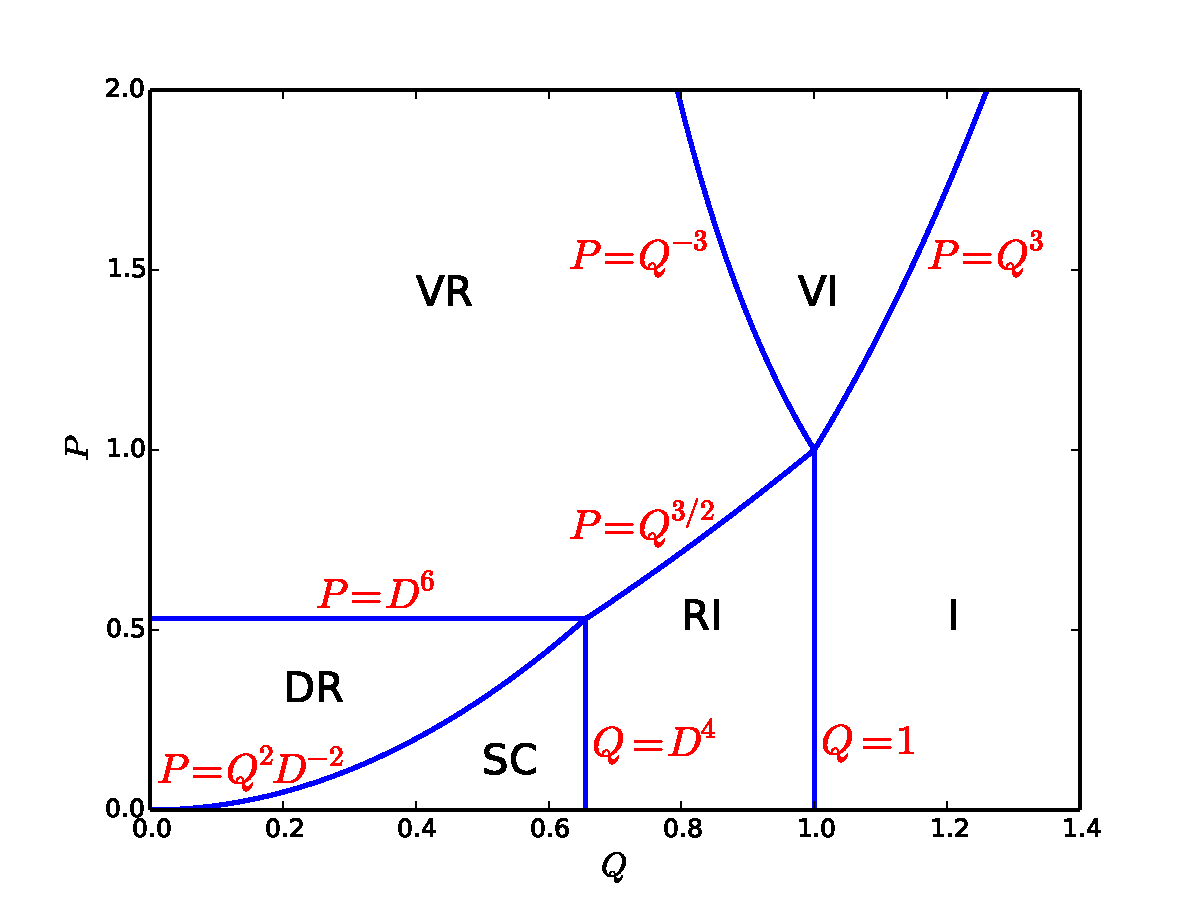
\includegraphics[width=0.95\textwidth]{Figure1.pdf}}
\caption{Linear resonant plasma response regimes in $Q$-$P$ space for the case $D=0.9$. The various regimes are
the diffusive-resisitive (DR), the semi-collisional (SC), the resistive-inertial (RI), the viscous-resistive (VR), the viscous-inertial
(VI), and the inertial (I).}\label{f1}
\end{figure}

\begin{figure}
\centerline{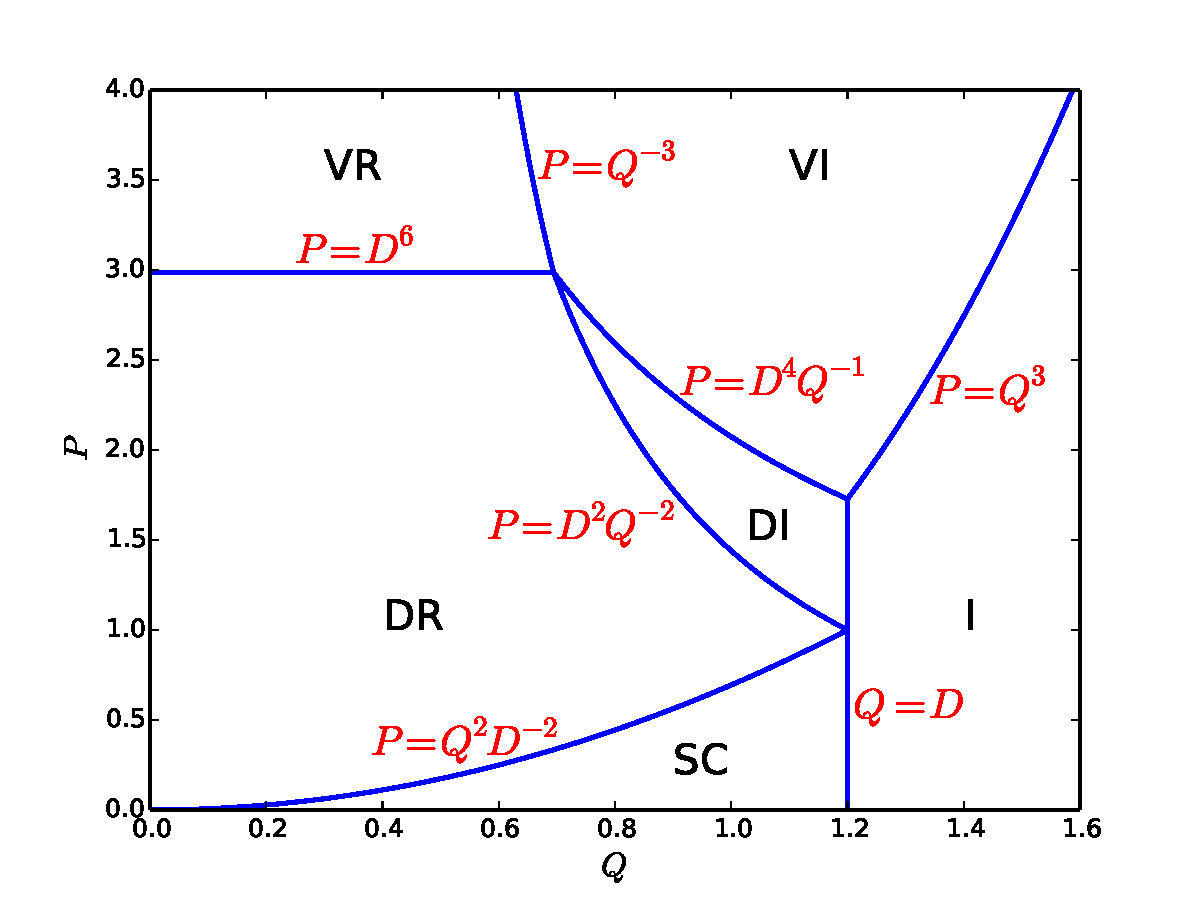
\includegraphics[width=0.95\textwidth]{Figure2.pdf}}
\caption{Linear resonant plasma response regimes in $Q$-$P$ space for the case $D=1.2$. The various regimes are
the diffusive-resisitive (DR), the semi-collisional (SC), the diffusive-inertial (DI), the viscous-resistive (VR), the viscous-inertial
(VI), and the inertial (I).}\label{f2}
\end{figure}

\begin{figure}
\centerline{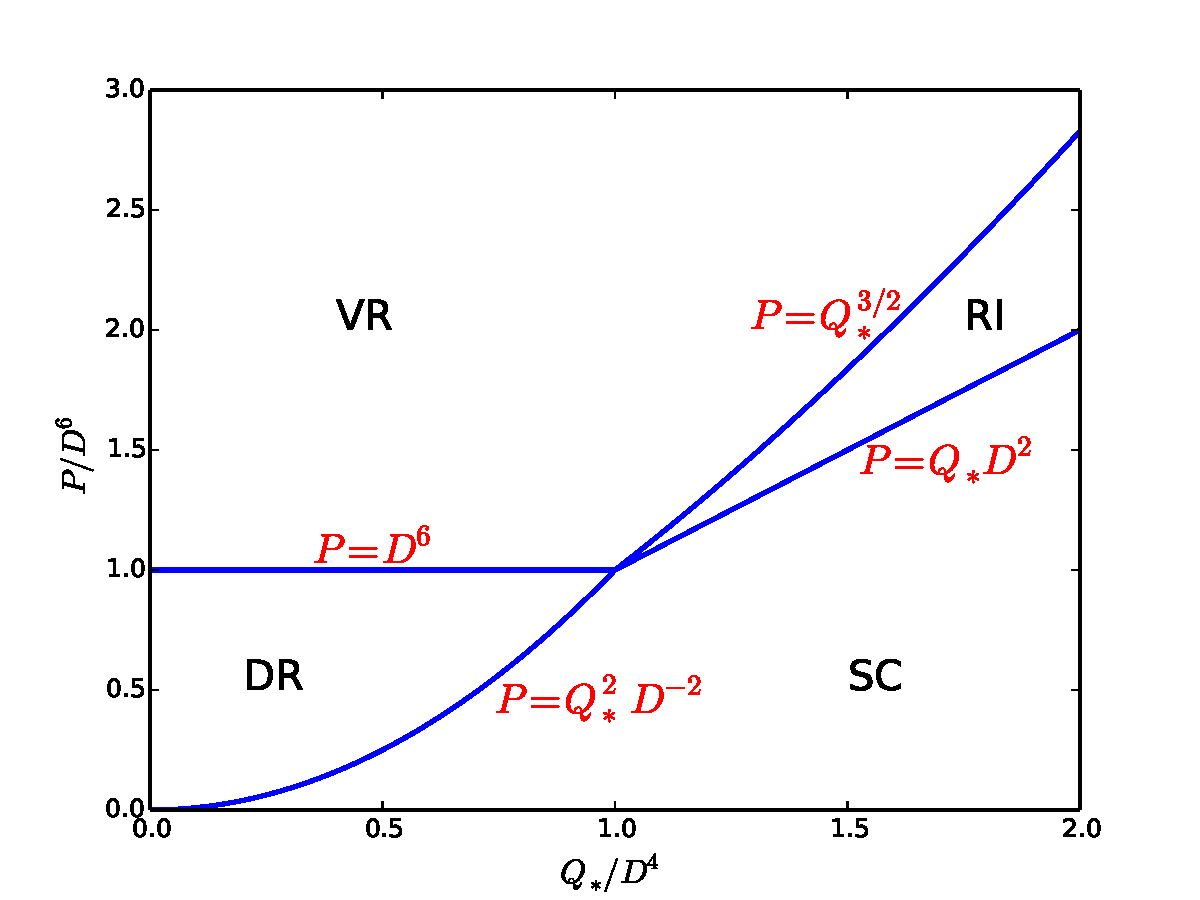
\includegraphics[width=0.95\textwidth]{Figure3.pdf}}
\caption{Linear tearing mode growth-rate regimes  in $Q_\ast$-$P$ space. The various regimes are
the diffusive-resisitive (DR), the semi-collisional (SC),  the viscous-resistive (VR), and the resistive-inertial (RI).}\label{f3}
\end{figure}

\begin{figure}
\centerline{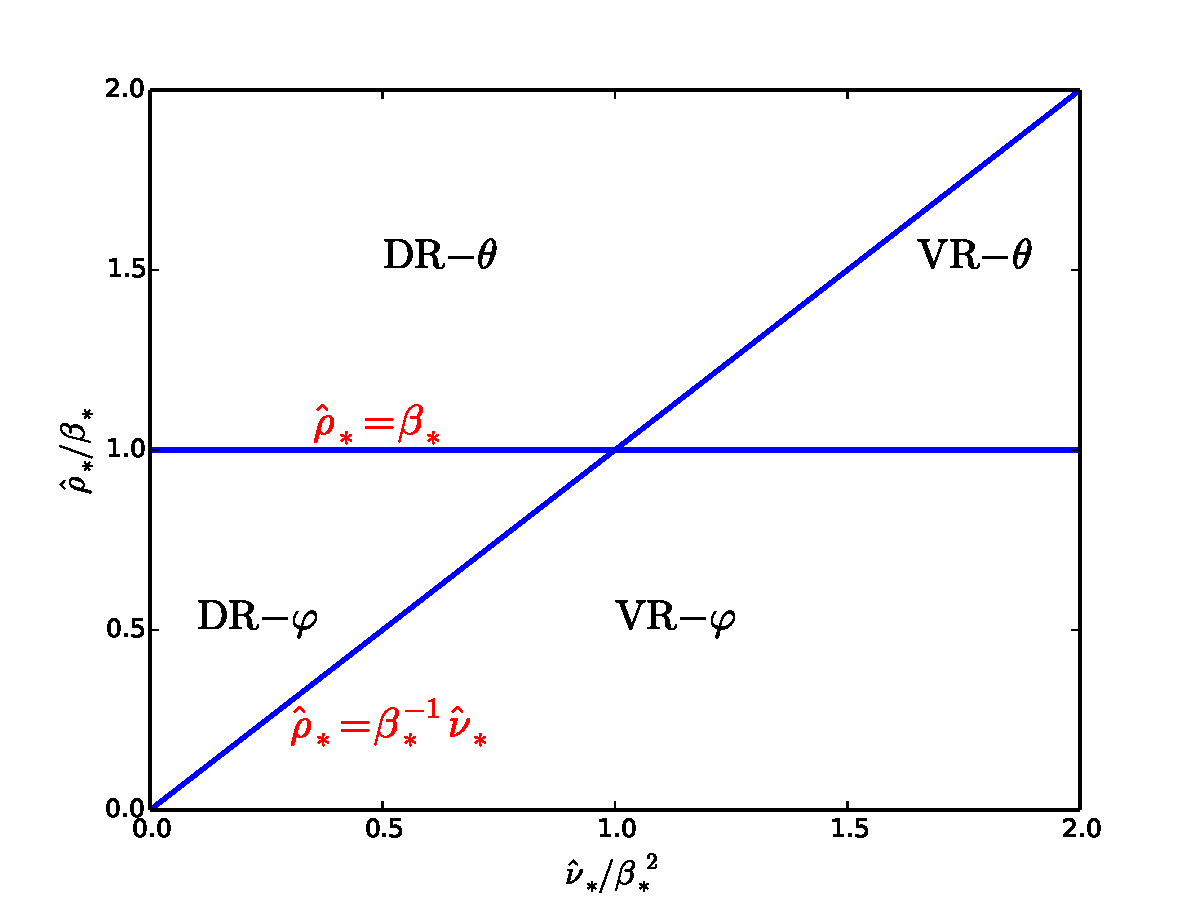
\includegraphics[width=0.95\textwidth]{Figure4.pdf}}
\caption{Error-field penetration regimes in $\hat{\nu}_\ast$-$\hat{\rho}_\ast$ space. The various regimes are the
viscous-resistive-toroidal (${\rm VR}$-$\varphi$), the viscous-resistive-poloidal (${\rm VR}$-$\theta$), the diffusive-resistive-poloidal (${\rm DR}$-$\theta$), and the  diffusive-resistive-toroidal (${\rm DR}$-$\varphi$). }\label{f6}
\end{figure}

\end{document}